% !TeX spellcheck = de_DE
% !TeX encoding = UTF-8
\documentclass{scrartcl}
%%%%%%%%%%%%%%%%%%%%%%%%%%%%%%%%%%%%%%%%%%%%%%%%%%%%%%%%%%%%%%%%%%%%%%%%%%%%%%%%%%%%%%%%%%%%%%%%%%%%%%%%%%%%%%%%%%%%%%%%%%%%%%%%%%%%%%%%%%%%%%%%%%%%%%%%%%%%%%%%%%%%%%%%%%%%%%%%%%%%%%%%%%%%%%%%%%%%%%%%%%%%%%%%%%%%%%%%%%%%%%%%%%%%%%%%%%%%%%%%%%%%%%%%%%%%
%\usepackage{answers} % Lösungen werden in Datei ans.tex gespeichert, aber nicht angezeigt. Ganz unten im Dokument kann man die Lösungen auch einbinden.
\usepackage[nosolutionfiles]{answers} %Lösungen werden direkt bei Aufgabe angezeigt
%%%%%%%%%%%%%%%%%%%%%%%%%%%%%%%%%%%%%%%%%%%%%%%%%%%%%%%%%%%%%%%%%%%%%%%%%%%%%%%%%%%%%%%%%%%%%%%%%%%%%%%%%%%%%%%%%%%%%%%%%%%%%%%%%%%%%%%%%%%%%%%%%%%%%%%%%%%%%%%%%%%%%%%%%%%%%%%%%%%%%%%%%%%%%%%%%%%%%%%%%%%%%%%%%%%%%%%%%%%%%%%%%%%%%%%%%%%%%%%%%%%%%%%%%%%%
\Newassociation{solution}{Solution}{ans}
\usepackage[T1]{fontenc}
\usepackage[utf8]{inputenc}
\usepackage{amssymb,amsmath,amsfonts}
\usepackage[ngerman]{babel}
\usepackage[a4paper,bottom=1.5in,top=1.5in]{geometry}
\usepackage{csquotes}
\usepackage{pdfsync}
\usepackage{enumerate}
\usepackage{graphicx}
\usepackage{hyperref}
\hypersetup{
pdfauthor={Willi Mutschler},
pdftitle={Einführung in die Makroökonomik},
pdfsubject={},
pdfproducer={LaTeX},
colorlinks=false,       pdfstartview={FitH},   plainpages = false, }
\usepackage{multicol}
\begin{document}

\title{Einführung in die Makroökonomik}
\subtitle{Version \today}
\author{Dr. Willi Mutschler\\willi@mutschler.eu}
\date{}
\maketitle
\newpage
\tableofcontents
\newpage
\section{Volkswirtschaftliche Gesamtrechnung}
\setcounter{page}{1}
\subsection{Verst\"{a}ndnis}

Erl\"{a}utern Sie die Prinzipien der VGR. Gehen Sie dabei auf folgende Punkte ein:
\begin{itemize}
  \item Was ist das BIP?
  \item Entstehungs, Verwendungs- und Verteilungsrechung,
  \item Strom- und Bestandsgr\"{o}{\ss}en,
  \item Akteure, die betrachtet werden,
  \item Besonderheiten einer offenen Volkswirtschaft,
  \item Inlands- und Inl\"{a}nderkonzept
  \item Finanzierungssaldos.
\end{itemize}
\subsection{Einfache Berechnungen}
Aus der VGR sind folgenden Daten jeweils in Mrd. EUR bekannt:
\begin{itemize}
\item Produktionswert zu Herstellungspreisen: 5.000
\item Vorleistungen: 2.700
\item G\"{u}tersteuern: 580
\item G\"{u}tersubventionen: 30
\item Bruttoinvestitionen: 870
\item Privater Konsum: 1.000
\item Staatskonsum: 500
\item Importe: 770
\item Abschreibungen: 450
\item Saldo Primäreinkommen mit dem Ausland: – 40
\end{itemize}
Berechnen Sie: das Bruttoinlandsprodukt, den Au{\ss}enbeitrag, die Exporte, die Nettoinvestitionen, das Bruttonationaleinkommen und das Nettonationaleinkommen.
\subsection{Berechnungen (I)}
Wie berechnet man, ausgehend vom Nettonationaleinkommen zu Faktorkosten, die Bruttoinvestitionen? Geben Sie für die nachfolgend genannten Größen der VGR jeweils an, ob sie vom Ausgangswert ausgehend addiert (+), subtrahiert (-) oder gar nicht berücksichtigt (0) werden müssen.\\~\\
\begin{tabular}{ll}
	Volkseinkommen & \\
	$\qquad\bullet$ Nettoinvestitionen &  \_\_\_\_ \\
	$\qquad\bullet$ Privater Konsum &  \_\_\_\_ \\
	$\qquad\bullet$ Indirekte Steuern &  \_\_\_\_ \\
	$\qquad\bullet$ Subventionen &  \_\_\_\_ \\
	$\qquad\bullet$ Gesamtwirtschaftlicher Konsum &  \_\_\_\_ \\
	$\qquad\bullet$ Direkte Steuern &  \_\_\_\_ \\
	$\qquad\bullet$ Abschreibungen &  \_\_\_\_ \\
	$\qquad\bullet$ Saldo der Primäreinkommen &  \_\_\_\_ \\
	$\qquad\bullet$ Außenbeitrag &  \_\_\_\_ \\
	= Bruttoinvestitionen  &
\end{tabular}

\subsection{Berechnungen (II)}
Wie berechnet man, ausgehend vom Privaten Verfügbaren Einkommen, das Nettonationaleinkommen zu Marktpreisen? Geben Sie für die nachfolgend genannten Größen der VGR jeweils an, ob sie vom Ausgangswert ausgehend addiert (+), subtrahiert (-) oder gar nicht berücksichtigt (0) werden müssen.\\~\\
\begin{tabular}{ll}
	Privates Verfügbares Einkommen & \\
	$\qquad\bullet$ Private Ersparnis &  \_\_\_\_ \\
	$\qquad\bullet$ Privater Konsum &  \_\_\_\_ \\
	$\qquad\bullet$ Saldo der laufenden Übertragungen &  \_\_\_\_ \\
	$\qquad\bullet$ Indirekte Steuern &  \_\_\_\_ \\
	$\qquad\bullet$ Subventionen &  \_\_\_\_ \\
	$\qquad\bullet$ Gesamtwirtschaftlicher Konsum &  \_\_\_\_ \\
	$\qquad\bullet$ Direkte Steuern &  \_\_\_\_ \\
	$\qquad\bullet$ Abschreibungen &  \_\_\_\_ \\
	$\qquad\bullet$ Saldo der Primäreinkommen &  \_\_\_\_ \\
	$\qquad\bullet$ Staatliche Ersparnis &  \_\_\_\_ \\
	= Nettonationaleinkommen zu Marktpreisen  &
\end{tabular}
\newpage
\subsection{Berechnungen (III)}
Wie berechnet man, ausgehend vom Bruttonationaleinkommen zu Marktpreisen, den Produktionswert zu Herstellungspreisen? Geben Sie für die nachfolgend genannten Größen der VGR jeweils an, ob sie vom Ausgangswert ausgehend addiert (+), subtrahiert (-) oder gar nicht berücksichtigt (0) werden müssen.\\~\\
\begin{tabular}{ll}
	Bruttonationaleinkommen zu Marktpreisen & \\
	$\qquad\bullet$ Nettoinvestitionen &  \_\_\_\_ \\
	$\qquad\bullet$ Privater Konsum &  \_\_\_\_ \\
	$\qquad\bullet$ Gütersteuern &  \_\_\_\_ \\
	$\qquad\bullet$ Primäreinkommen aus dem Ausland &  \_\_\_\_ \\
	$\qquad\bullet$ Gütersubventionen &  \_\_\_\_ \\
	$\qquad\bullet$ Gesamtwirtschaftlicher Konsum &  \_\_\_\_ \\
	$\qquad\bullet$ Vorleistungen &  \_\_\_\_ \\
	$\qquad\bullet$ Direkte Steuern &  \_\_\_\_ \\
	$\qquad\bullet$ Abschreibungen &  \_\_\_\_ \\
	$\qquad\bullet$ Saldo der Primäreinkommen &  \_\_\_\_ \\
	$\qquad\bullet$ Außenbeitrag &  \_\_\_\_ \\
	= Produktionswert zu Herstellungspreisen  &
\end{tabular}

\subsection{Berechnungen (IV)}
Wie berechnet man, ausgehend vom Verfügbaren Einkommen der Gesamtwirtschaft, die Bruttoinvestitionen? Geben Sie für die nachfolgend genannten Größen der VGR jeweils an, ob sie vom Ausgangswert ausgehend addiert (+), subtrahiert (-) oder gar nicht berücksichtigt (0) werden müssen.\\~\\
\begin{tabular}{ll}
	Verfügbares Einkommen der Gesamtwirtschaft& \\
	$\qquad\bullet$ Primäreinkommen aus dem Ausland &  \_\_\_\_ \\
	$\qquad\bullet$ Nettoinvestitionen &  \_\_\_\_ \\
	$\qquad\bullet$ Gesamtwirtschaftlicher Konsum &  \_\_\_\_ \\
	$\qquad\bullet$ Indirekte Steuern &  \_\_\_\_ \\
	$\qquad\bullet$ Laufende Übertragungen aus der ÜW &  \_\_\_\_ \\
	$\qquad\bullet$ Laufende Übertragungen an die ÜW &  \_\_\_\_ \\
	$\qquad\bullet$ Direkte Steuern &  \_\_\_\_ \\
	$\qquad\bullet$ Abschreibungen &  \_\_\_\_ \\
	$\qquad\bullet$ Primäreinkommen an das Ausland &  \_\_\_\_ \\
	$\qquad\bullet$ Außenbeitrag &  \_\_\_\_ \\
	= Bruttoinvestitionen  &
\end{tabular}
\newpage
\subsection{Kreislaufschema (I)}
Errechnen Sie für das hier dargestellte Kreislaufschema einer offenen Volkswirtschaft mit Staat die Werte für den Privaten Konsum, das Volkseinkommen, das Finanzierungssaldo der Unternehmen und das Finanzierungssaldo der übrigen Welt.\\~\\
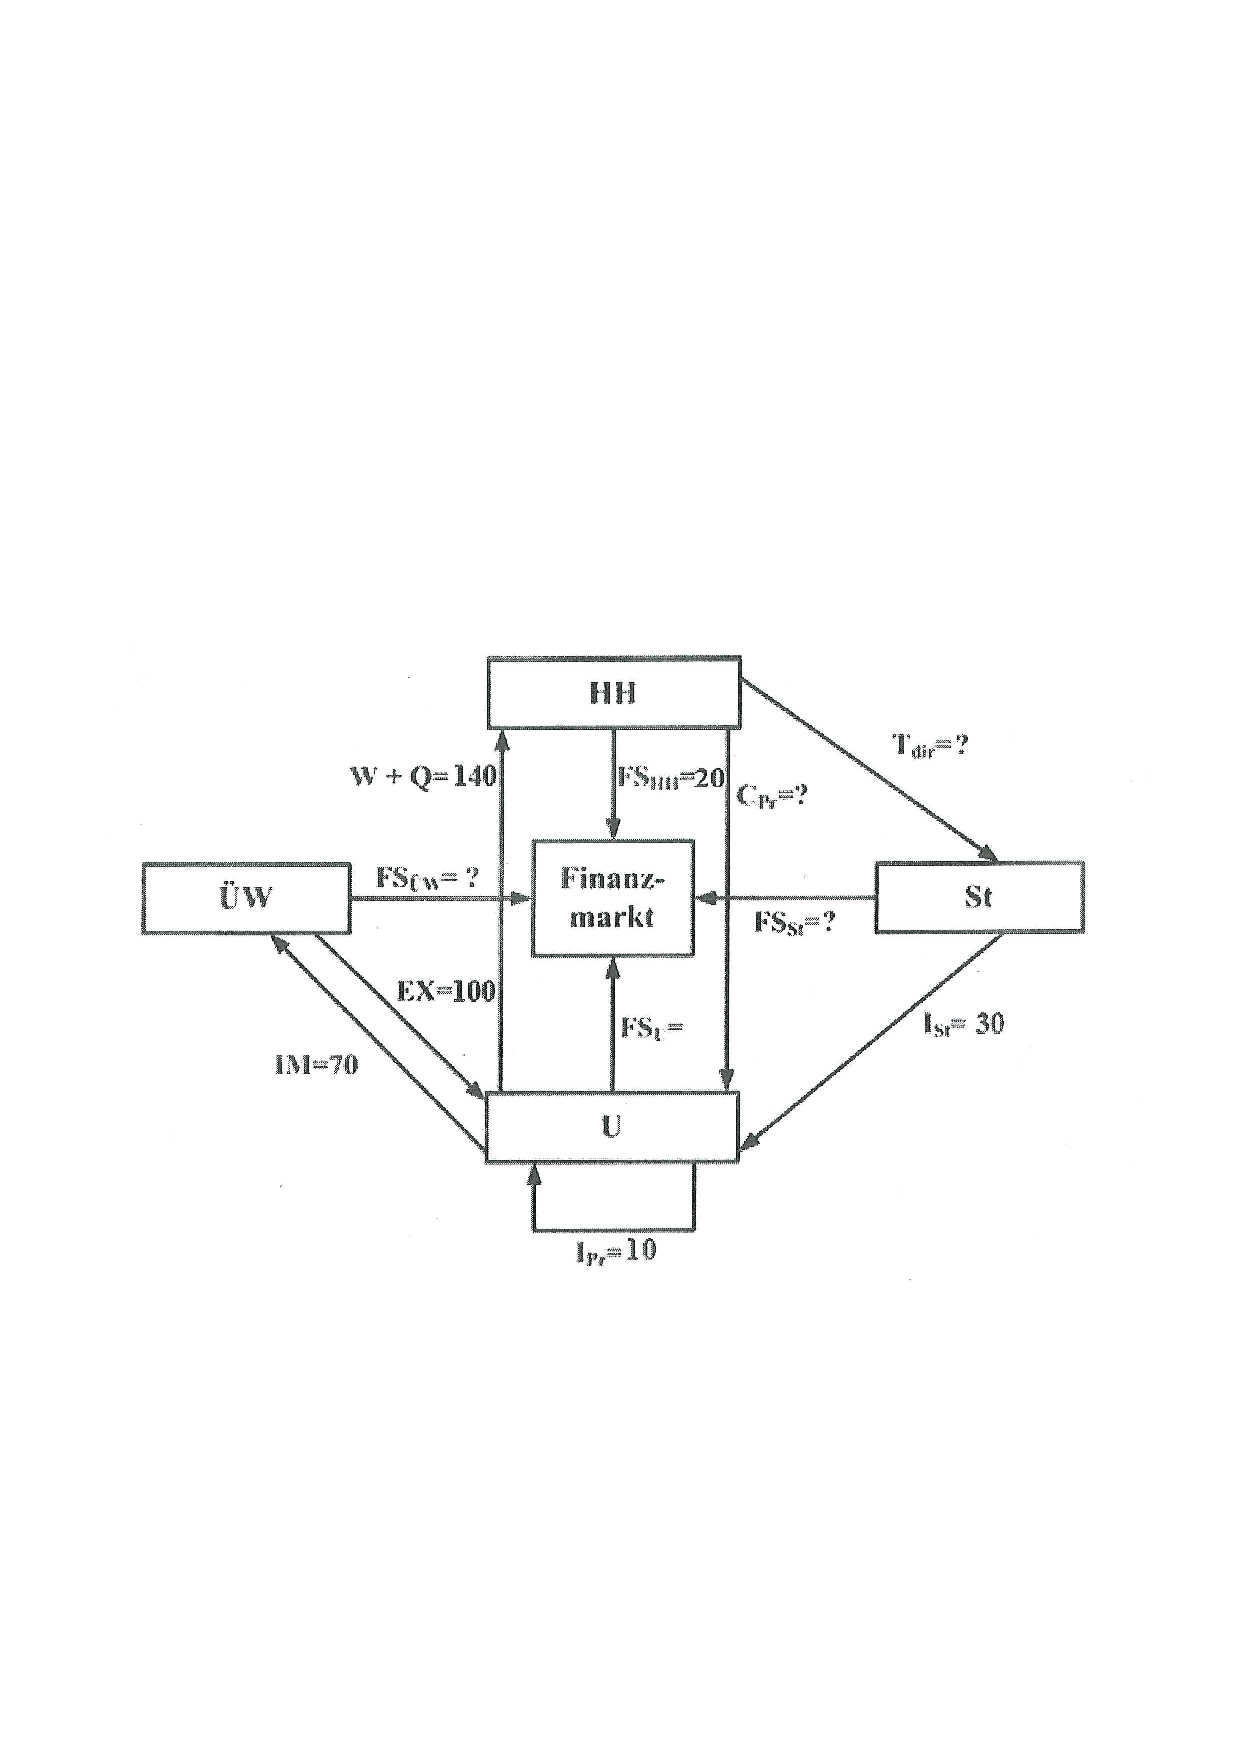
\includegraphics[width=\textwidth]{Bilder/Klassik_Kreislauf_Diagramm_Aufgabe.pdf}

\subsection{Kreislaufschema (II)}
Fertigen Sie ein Kreislaufdiagramm für eine offene Volkswirtschaft mit staatlicher Aktivität an. Der private Konsum betrage 160, der Finanzierungssaldo der Unternehmen betrage -60, die staatlichen Investitionen 20, der Finanzierungssaldo des Staates betrage 20, die Exporte 80 und die Importe 120. Vervollständigen Sie das Kreislaufdiagramm um die direkten Steuern, den Finanzierungssaldo der Haushalte und der übrigen Welt und der Summe aus Lohn – und Gewinnzahlungen der Unternehmen.

\subsection{Finanzierungssalden}
In einer geschlossenen Ökonomie ohne indirekte Steuern, Subventionen und Abschreibungen bezeichne Y das BIP, C den Konsum, I die Investitionen, G die Staatsausgaben, T die direkten Steuern und TR die staatlichen Transfers.
\begin{enumerate}
	\item Wie ist der Finanzierungssaldo im Allgemeinen definiert? Bestimmen Sie den Finanzierungssaldo der Haushalte, der Unternehmen und des Staates.
	\item Wie hoch ist die Summe der Finanzierungssalden? Geben Sie eine ökonomisch-intuitive Erklärung, warum das so ist.
\end{enumerate}

\subsection{Geschlossene vs. Offene Volkswirtschaft}
In einer geschlossenen Ökonomie bezeichne BIP das Bruttoinlandsprodukt, Y das Volkseinkommen, C den privaten Konsum, I die privaten Investition und G den Staatskonsum. Nehmen Sie vereinfachend an, dass die Abschreibungen, die indirekten und direkten Steuern, Subventionen und Transfers gleich Null sind.
\begin{enumerate}
	\item Wie lautet der Zusammenhang zwischen BIP und Y? Warum ist dies so?
	\item Welcher Zusammenhang besteht zwischen privater Ersparnis und Staatsverschuldung?
	\item Betrachten Sie nun eine offene Ökonomie. Welcher Zusammenhang besteht hier zwischen privater Ersparnis und Außenbeitrag?
\end{enumerate}

\subsection{Verst\"{a}ndnisfragen (wahr/falsch)}
\begin{enumerate}
  \item Das Nettonationaleinkommen zu Marktpreisen ergibt sich als Bruttonationaleinkommen zu Marktpreisen minus Abschreibungen.% (wahr)
  \item Die in der VGR erfasste Ersparnis stellt, \"{a}hnlich wie die Ersparnis auf einem Bankkonto, eine Bestandsgr\"{o}{\ss}e dar.% (falsch)
  \item In einer offenen Volkswirtschaft ist es m\"{o}glich, dass ex post gesamtwirtschaftlich das Sparen positiv ist, die Nettoinvestition aber gleich Null ist.% (wahr)
  \item Wenn die Abschreibung eines Unternehmens gr\"{o}{\ss}er ist als dessen Nettowertsch\"{o}pfung, dann nimmt die Bruttowertsch\"{o}pfung einen negativen Wert an.% (falsch)
  \item Im Kontensystem der VGR gibt das Einkommenskonto Auskunft dar\"{u}ber, welche Einkommen ein Wirtschaftssubjekt erh\"{a}lt und wozu es diese Einkommen verwendet.% (wahr)
  \item In einer geschlossenen Volkswirtschaft gilt stets, dass ex post der Finanzierungssaldo gleich Null ist. % (wahr)
  \item In einer offenen Volkswirtschaft kann das Nettonationaleinkommen niemals kleiner sein als das Nettoinlandsprodukt% (falsch)
  \item In einer offenen Volkswirtschaft entspricht die H\"{o}he des Nettonationaleinkommens stets der H\"{o}he des Volkseinkommens% (falsch)
  \item Das Bruttonationaleinkommen wird nach dem Inlandskonzept bemessen. % (falsch)
    \item Das Bruttoinlandsprodukt ist stets gr\"{o}{\ss}er als das Nettonationaleinkommen. %(falsch)
  \item Bei der Verteilungsrechnung ist der Ausgangspunkt die Verteilung des Konsums von privaten und \"{o}ffentlichen Haushalten sowie der Investitionen des Staates% (falsch)
    \item Die Nettoinvestitionen sind entweder positiv oder gleich null. %(falsch)
  \item Wenn in einem Land ex post die gesamtwirtschaftliche Ersparnis kleiner ist als die gesamtwirtschaftlichen Investitionen, so mu{\ss} es zu einem Nettokapitalimport gekommen sein. %(wahr)
  \item Wenn in einer \"{O}konomie die Nettoinvestition der Ersparnis entspricht, so kann es sich
um eine geschlossene Volkswirtschaft handeln. %(wahr)
\item \"{U}bersteigen die Bruttoinvestitionen die Abschreibungen, so sind die Reinvestitionen in einer Periode stets genauso gro{\ss} wie die Abschreibungen. %(wahr)
\item Auch in der offenen Volkswirtschaft k\"{o}nnen sich die gesamtwirtschaftliche Ersparnis
und die inl\"{a}ndischen Investitionen entsprechen. %(wahr)
\item In einer geschlossenen Volkswirtschaft kann es sowohl Gl\"{a}ubiger, als auch Schuldner
geben. Gesamtwirtschaftlich ist der aggregierte Bondbestand jedoch stets gleich null. %(wahr)

\end{enumerate}

\subsection{Lohnquote}
Berechnen Sie auf Basis der folgenden Angaben f\"{u}r eine Phantasievolkswirtschaft die (unbereinigte) Bruttolohnquote:
\begin{itemize}
  \item Bruttonationaleinkommen: 2000
  \item Nettol\"{o}hne und -geh\"{a}lter: 900
  \item Bruttol\"{o}hne und -geh\"{a}lter: 1100
  \item Arbeitgeberbeitr\"{a}ge zur Sozialversicherung: 300
  \item Arbeitnehmerbeitr\"{a}ge zur Sozialversicherung: 200
  \item Anzahl der Arbeitnehmer: 120000
  \item Anzahl der Selbst\"{a}ndigen: 30000
  \item Au{\ss}enbeitrag: -400
  \item Konsumausgaben der Haushalte: 1200
  \item Saldo der Prim\"{a}reinkommen aus dem Ausland: -10
  \item Abschreibungen: 300
\end{itemize}
Wie \"{a}ndert sich diese Gr\"{o}{\ss}e, wenn
\begin{itemize}
\item[(a)] der Anteil der Selbst\"{a}ndigen unter den Erwerbspersonen steigt,
\item[(b)] die Arbeitnehmerbeitr\"{a}ge zur Sozialversicherung steigen,
\item[(c)] die Konsumausgaben der Haushalte fallen?
\end{itemize}
\subsection{Lorenzkurve + Gini-Koeffizient}
Betrachten Sie eine Modell\"{o}konomie, die aus f\"{u}nf blauen und f\"{u}nf gr\"{u}nen Personen bewohnt wird. Jede gr\"{u}ne Person hat ein Einkommen von 1 pro Periode, und jede blaue Person hat ein Einkommen von 3 pro Periode. Zeichnen Sie die Lorenzkurve f\"{u}r diese \"{O}konomie und berechnen Sie den Gini-Koeffizienten.

\subsection{BIP-Konzepte: Nominal, Real, Kettenindex}
Die folgende Tabelle beschreibt die Entwicklung des realen Bruttoinlandsproduktes (BIP), gemessen
in Mrd. Euro und in Preisen von 2005, sowie die Werte des Kettenindex:
\begin{center}
\begin{tabular}{|c|c|c|}
  \hline
   & Reales BIP & Kettenindex \\
  2005 & 2224 & 100 \\
  2006 & 2231 & 103,7 \\
  2007 & 2267 & 107,1 \\
  \hline
\end{tabular}
\end{center}
\begin{enumerate}[a)]
  \item Erl\"{a}utern Sie den Unterschied zwischen nominalem und realem BIP. Gehen Sie dabei auch auf das Konzept des Kettenindex ein.
  \item Berechnen Sie f\"{u}r die Jahre 2005, 2006 und 2007 das nominale BIP.
  \item Berechnen Sie die Wachstumsrate des realen BIP zum jeweiligen Vorjahr in Prozent.
  \item Berechnen Sie die Wachstumsrate des realen BIP \"{u}ber die gesamte Periode in Prozent
  \item Berechnen Sie die mittlere j\"{a}hrliche Wachstumsrate des realen BIP \"{u}ber die gesamte Periode.
\end{enumerate}

\subsection{Klausuraufgaben}
\begin{enumerate}
  \item Definieren Sie den Begriff \emph{Bruttoinlandsprodukt}.
  \item Wie kommt man vom Bruttoinlands- zum Nettoinladsprodukt? Erl\"{a}utern Sie den Unterschied.
  \item Grenzen Sie das Bruttoinlandsprodukt gegen\"{u}ber dem Bruttonationaleinkommen, dem Nettonationaleinkommen, dem Volkseinkommen, sowie dem verf\"{u}gbaren Einkommen der privaten Haushalte ab. F\"{u}r welche Fragestellungen sind die unterschiedlichen Einkommenskonzepte jeweils besonders aussagekr\"{a}ftig?
  \item Erl\"{a}utern Sie den Unterscheid zwischen Entstehungs-, Verwendungs- und Verteilungsrechnung.
  \item Nennen Sie 3 Argumente, die das BIP als Wohlstandsindikator ungeeignet erscheinen lassen.
  \item Erl\"{a}utern Sie ein Konzept zur alternativen Wohlstandsmessung. Wie vergleicht sich dieses mit dem BIP als Wohlstandsindikator?
  \item Warum ist das BIP in einem Land wie Irland höher als das BNE?
  \item Gegeben sei eine Volkswirtschaft, deren Bewohner sich ausschließlich von Pommes und Kartoffelchips ernähren. In diesem Land gebe es 3 Unternehmen: ein Kartoffeln anbauender landwirtschaftlicher Betrieb, eine Pommes-Fabrik und ein Hersteller von Kartoffelchips. Die Unternehmen weisen folgende Gewinn- und Verlustrechnung aus:
  \begin{center}
  \begin{tabular}{|c|c|c|c|}
  	\hline 
  	&Landwirtschaft  &Pommes-Fabrik  &Chips-Produzenten  \\ 
  	\hline 
  	Verkaufserlöse&600  & 2000  & 400 \\ 
  	\hline 
  	Einkäufe bei der Landwirtschaft& -  &500  & 100 \\ 
  	\hline 
  	Löhne& 440 & 1200  & 260  \\ 
  	\hline 
  	Gewinne &160  &300  &40  \\ 
  	\hline 
  \end{tabular}\end{center}
\noindent Berechnen Sie das BIP dieser Volkswirtschaft mittels der Entstehungs-, Verwendungs- und Verteilungsrechnung und erläutern Sie ihr Vorgehen verbal. 
\end{enumerate}
\newpage
\section{Die (Neo-)Klassische Theorie}

\subsection{Verständnis}
\begin{enumerate}
	\item Erläutern Sie die Begriffe des repräsentativen Unternehmens und des repräsentativen Haushalts. Gehen Sie dabei auf das Gewinnmaximierungskalkül des Unternehmens sowie die Budgetrestriktion und das Optimierungskalkül des Haushaltes formal ein. Warum hängt die Arbeitsnachfragefunktion des repräsentativen Unternehmens negativ und das Arbeitsangebot des repräsentativen Haushalts positiv vom Reallohnsatz ab?
	\item Beschreiben Sie den Arbeitsmarkt und erläutern Sie den Begriff der Vollbeschäftigung im klassisch-neoklassischen Modell.
	\item Beschreiben Sie den Kapitalmarkt und erläutern Sie, warum im Kapitalmarktgleichgewicht der Zins mit der Grenzproduktivität des Kapitals übereinstimmt. Nehmen sie hierzu an, dass mit steigendem Zins die Ersparnis zunimmt.
	\item Beschreiben Sie den Gütermarkt und erläutern Sie in diesem Zusammenhang das Gesetz von Walras.
	\item Unterscheiden Sie die Quantitätsgleichung von der Quantitätstheorie. Erläutern sie hierbei den Cambridge-Effekt.
	\item Leiten Sie grafisch die Güterangebotsfunktion her. Erläutern Sie deren Verlauf.
	\item Leiten Sie das klassisch-neoklassische Gesamtmodell graphisch her und erläutern Sie den Begriff der Dichotomie. Wann verschieben sich die Kurven?
	\item Erweitern Sie das Modell um den Staatssektor und zeigen Sie den Einfluss einer
	\begin{enumerate}[(i)]
		\item Kreditfinanzierten Staatsausgabenerhöung
		\item Steuerfinanzierten Staatsausgabenerhöung
		\item Erhöhung des Geldangebots
	\end{enumerate}
	Nehmen sie hierzu an, dass mit steigendem Zins die Ersparnis zunimmt. Erläutern Sie in diesem Zusammenhang das Konzept des Crowding-Outs. Was ändert sich, wenn die Ersparnis unabhängig vom Zins ist?
\end{enumerate}
\subsection{Rechenaufgabe}
Die Produktionsfunktion des Unternehmenssektors eines Landes sei gegeben durch:
\begin{align*}
Y = F(N) = 4 \sqrt{N}
\end{align*}
Die Arbeitsangebotsfunktion sei gegeben durch $N^s = 3 -\frac{4}{\left(\frac{w}{p}\right)}$. Dabei sei das Preisniveau auf 1 normiert.
\begin{enumerate}
	\item Leiten Sie die Arbeitsnachfragefunktion $N^d$ ab.
	\item Bestimmen Sie den gleichgewichtigen Reallohnsatz, die Beschäftigung im Gleichgewicht, die produzierte Gütermenge, die Lohnsumme, die Lohnquote und den Gewinn im Gleichgewicht.
\end{enumerate}

\subsection{Kassenhaltungskoeffizient im (neo-)klassischen Modell}
In der (neo-)klassischen Modellwelt möge der Kassenhaltungskoeffizient $k=1/v$ sinken. Welche Auswirkungen hat dies auf die endogenen Variablen im neuen, langfristigen Gleichgewicht? Inwiefern ändern sich ihre Ergebnisse bei einem starren Nominallohn?
\subsection{Nominallohn im (neo-)klassischen Modell}
In der (neo-)klassischen Modellwelt möge der Nominallohn sinken. Welche Auswirkungen hat dies auf die endogenen Variablen im neuen, langfristigen Gleichgewicht? Inwiefern ändern sich ihre Ergebnisse bei einem starren Nominallohn, d.h. der starre Nominallohn möge einmalig sinken?

\subsection{Kapitalstock und Geldpolitik im (neo-)klassischen Modell}
Analysieren Sie grafisch, welche Auswirkung ein steigender Kapitalstock im Rahmen des klassischen Modells auf das Gleichgewicht der Ökonomie hat. Inwiefern ändern sich ihre Ergebnisse bei einem starren Nominallohn?

\subsection{Verständnisfragen (wahr/falsch)}
\begin{enumerate}
	\item Die Budgetrestriktion eines Haushaltes beschreibt alle möglichen Kombinationen von Einkommen, Konsum, Bargeld- und Bondhaltung, für die der Haushalt indifferent ist. (wahr)
	\item Im Fall eines positiven Angebotsschocks, der die Produktionsfunktion proportional nach oben verschiebt, wollen die Wirtschaftssubjekte stets weniger arbeiten. (falsch)
	\item Im klassisch-neoklassischen Modell führt eine Zunahme der Geldmenge nicht zu einer Veränderung des realen Niveaus von Output und Konsum im Gleichgewicht. (wahr)
	\item Nehmen Sie an, auf dem Arbeitsmarkt herrsche bei gegebenem Reallohnsatz ein Überschussangebot. Beim gegebenen Reallohnsatz herrscht also Arbeitslosigkeit. (wahr)
	\item Im neoklassischen Modell steigen (ceteris paribus) die Nettoinvestitionen immer dann, wenn der reale Zinssatz sinkt. (wahr)
	\item Im klassisch-neoklassischen Modell ist der Zinssatz der Preis des Geldes. Daher muss zur Räumung des Geldmarktes der Zins sinken, wenn auf dem Geldmarkt eine Überschußnachfrage herrscht. (falsch)
	\item Die Konsumnachfrage hängt im klassisch-neoklassischen Modell mit Zinsabhängiger Ersparnis negativ vom Zins ab, da mit steigendem Zins der Konsum in der heutigen Periode gegenüber dem Konsum in der zukünftigen Periode teurer wird. (wahr)
	\item Herrscht im klassisch-neoklassischen Modell Arbeitslosigkeit, so besteht auf dem Arbeitsmarkt eine Überschussnachfrage. (falsch)
	\item Im Fall einer Staatsausgabenerhöhung versteht man in einer geschlossenen Volkswirtschaft unter „crowding out“, daß diese zusätzlichen Ausgaben des Staates private Investitionen und Konsum verdrängen. (wahr)
	\item Gemäß dem „Crowding-Out-Effekt“ führt ein Anstieg des staatlichen Budgetdefizits zu einer Verringerung der privaten Investitionen, da der reale Zinssatz sinkt. (falsch)
	\item Wenn Geldmarkt und Gütermarkt im Gleichgewicht sind, dann sind es auch Kreditmarkt und Arbeitsmarkt. (falsch)
	\item Das Walras'sche Gesetz impliziert, dass nur eine gerade Anzahl von Märkten im Ungleichgewicht sein kann, da jedem Markt mit Überschußnachfrage ein Markt mit Überschußangebot gegenüberstehen muss. (falsch)
	\item Damit das Gesetz von Walras gilt, müssen alle betrachteten Märkte einer Volkswirtschaft geräumt sein. (falsch)
	\item Existieren in einer Volkswirtschaft 4 Märkte und sind davon 2 Märkte geräumt, so muss das Überschussangebot auf dem 3. Markt der Überschussnachfrage auf dem 4. Markt genau entsprechen. (wahr)
	\item Auf dem Geldmarkt und dem Gütermarkt herrsche Gleichgewicht, außerdem gibt es Arbeitslosigkeit. Damit das Gesetz von Walras gilt, muß auf dem Kreditmarkt ein Überschußangebot herrschen. (falsch)
	\item Bei Betrachtung dreier Märkte impliziert das Gesetz von Walras: Wenn auf einem Markt ein Überschussangebot und auf einem anderen Markt eine Überschussnachfrage herrscht, dann befindet sich der dritte Markt immer im Gleichgewicht. (falsch)
	\item Das Gesetz von Walras gilt nur dann, wenn die Wirtschaftspläne der Wirtschaftssubjekte von vornherein kompatibel sind. (falsch)
	\item Die Quantitätsgleichung besagt, dass die Umlaufgeschwindigkeit konstant ist. (falsch)
	\item Die Quantitätstheorie sagt, dass ein Sinken der Geldmenge langfristig ein sinkendes Sozialprodukt zur Folge hat. (falsch)
	\item Die Quantitätstheorie sagt, dass ein Anstieg der Geldmenge langfristig zu einem Anstieg des Preisniveaus führt. (wahr)
	\item Die Quantitätsgleichung zeigt die schädlichen Wirkungen der Inflation. (falsch)
	\item Die Quantitätstheorie zeigt die positiven Wirkungen der Inflation. (falsch)
	\item Die Quantitätsgleichung zeigt, dass ein Sinken der Geldmenge durch einen Anstieg der Umlaufgeschwindigkeit ausgeglichen werden könnte. (wahr)
	\item Nach der Quantitätstheorie ist die Geldmenge abhängig vom Sozialprodukt. (falsch)
	\item Wenn exogene Faktoren ein Sinken der Umlaufgeschwindigkeit verursachen, sinkt nach der Quantitätstheorie das Preisniveau. (wahr)
	\item Nach der Quantitätstheorie ist die Umlaufgeschwindigkeit abhängig vom Preisniveau. (falsch)
	\item Wenn die Notenbank die Geldmenge nicht erhöht, kommt es – laut der Quantitätstheorie – zu einem Sinken des Preisniveaus, wenn das Einkommen steigt. (wahr)
	\item Erhöht sich in der Quantitätsgleichung die Geldmenge, ist nicht eindeutig, ob die Umlaufsgeschwindigkeit fällt, die Preise steigen oder das Einkommen steigt. (wahr)
	\item Mittels der Quantitätstheorie können Aussagen darüber getroffen werden, wie sich die Geldmenge ändert, wenn das Preisniveau steigt. (falsch)
	\item Gemäß Quantitätsgleichung verdoppeln sich bei einer Geldmengenverdopplung zwangsläufig die Preise. (falsch)
	\item Gültigkeit der Quantitätstheorie vorausgesetzt gilt: Wenn die gesamtwirtschaftliche Konsumnachfrage steigt, steigt ceteris paribus das Preisniveau, da das Angebot konstant bleibt. (falsch)
	\item Gemäß Quantitätsgleichung folgt aus einer Erhöhung der Geldmenge immer ein proportionaler Anstieg des Preisniveaus. (falsch)
	\item Da die Quantitätstheorie lediglich aus einer Definitionsgleichung abgeleitet wird, können in ihrem Rahmen keine Aussagen über kausale Zusammenhänge gemacht werden. (falsch)
	\item Da die Quantitätsgleichung nur eine Identitätsgleichung ist, kann im Voraus nicht gesagt werden, welche Variable sich ändert, wenn sich eine der anderen Variablen ändert. (wahr)
	\item Gilt die Quantitätstheorie, ist das Einkommen immer fix. (falsch)
	\item Je höher der Kassenhaltungskoeffizient in einer Volkswirtschaft ist, desto geringer ist ceteris paribus die Umlaufsgeschwindigkeit. (wahr)
	\item Wenn Geld neutral ist, führt eine Verdopplung der nominalen Geldmenge zu einer Verdopplung des Preisniveaus, während das reale Einkommen konstant bleibt. (wahr)
	\item Das reale Geldangebot passt sich der realen Geldnachfrage nach der Quantitätstheorie dadurch an, dass sich das nominale Geldangebot anpasst. (falsch)
	\item Die Quantitätsgleichung sagt, dass immer dann, wenn die Geldmenge sinkt, das Preisniveau sinkt. (falsch)
	\item Handelsvolumen $\cdot$ Preisniveau = Geldmenge $\cdot$ Umlaufsgeschwindigkeit ist eine Identitätsgleichung, die immer gilt. (wahr)
\end{enumerate}

\newpage
\section{Keynesianische Theorie}
\subsection{Keynesianische Kreuz, Sparfunktion, und Multiplikatoren}
Gegeben sei folgendes Modell einer
geschlossenen Volkswirtschaft ohne staatliche Aktivität, in dem der \textbf{Zinssatz i exogen gegeben} ist:
\begin{align*}
&\text{Konsumfunktion: } &\quad& C = C_{aut} + c\cdot Y,\qquad 0\leq c \leq 1\\
&\text{Investitionsfunktion: } &\quad&I = I_{aut}-bi,\qquad b>0\\
&\text{Gesamtwirtschaftliche Güternachfrage: } &\quad&Y^d = C + I\\
&\text{Gleichgewichtsbedingung: } &\quad&Y^d = Y^s\\
&\text{Güterproduktion entspricht dem Volkseinkommen: } &\quad& Y^s = Y
\end{align*}

\begin{enumerate}[(a)]
  \item Erläutern Sie die fundamentalen Unterschiede der keynesianischen Theorie zur neoklassischen Theorie.
  \item Erl\"{a}utern Sie die einzelnen Gleichungen. Welche Variablen sind
      exogen, welche endogen? Gehen Sie auch auf das Verhalten der
      Haushalte und der Produzenten ein.
 \item Was versteht man unter der absoluten und permanenten Einkommenshypothese? Erläutern Sie kurz, wie beide Hypothesen die Konsumfunktion verändern. Gehen Sie kurz auf die wirtschaftspolitische Relevanz beider Hypothesen ein.
  \item Leiten Sie analytisch und graphisch die Sparfunktion ab.
      Bestimmen Sie die marginale Spar- und Konsumneigung.
  \item Bestimmen Sie graphisch und rechnerisch das gleichgewichtige
      Einkommen $Y^*$, indem Sie
      \begin{align*}
      (i)&~ Y=C+I\\
      (ii)&~ I=S
      \end{align*}
      setzen. In welchem Bereich darf die marginale Konsumneigung liegen, wenn ein sinnvolles Gleichgewicht existieren soll?
  \item Zeigen Sie graphisch und rechnerisch, wie eine Erh\"{o}hung des autonomen Konsums
  auf das gleichgewichtige Einkommen wirkt. Interpretieren Sie die
  Ergebnisse, und erkl\"{a}ren Sie den \textbf{Multiplikatorprozess}. Unter
  welchen Umst\"{a}nden kommt der Prozess zu einem Ende?
  \item Betrachten Sie nun das erweiterte Modell mit Staatst\"{a}tigkeit. Inwiefern \"{a}ndern sich die Modellgleichungen?
  \item Erl\"{a}utern Sie das Sparparadox im erweiterten Modell mit Staatst\"{a}tigkeit, in dem Sie drei F\"{a}lle betrachten:
  \begin{enumerate}[(i)]
  \item einen Kreditfinanzierten Anstieg der Staatsausgaben
  \item einen Steuerfinanzierten Anstieg der Staatsausgaben
  \item einen Anstieg der privaten autonomen Ersparnis
  \item die marginale Konsumquote sinkt
  \end{enumerate}
\end{enumerate}

\subsection{Haavelmo Theorem im Keynesianischen Modell}
Die Konsumfunktion in einer Ökonomie sei $C(Y_V)=C_{aut}+c Y_V$, die Investitionen $I_{aut}$ und die Staatsausgaben $G$ seien autonom. $Y_V$ ist das verfügbare Einkommen.
\begin{enumerate}
	\item Bestimmen Sie algebraisch das gleichgewichtige Einkommen.
	\item Zeigen Sie grafisch und algebraisch, welchen Effekt eine Staatsausgabenerhöhung auf das Einkommen im Gleichgewicht hat, wenn die Staatsausgabenerhöhung komplett durch eine einkommensunabhängige Steuer T gegenfinanziert wird. Erläutern Sie ihr Resultat kurz.
\end{enumerate}


\subsection{IS-Kurve}
Eine Volkswirtschaft sei durch folgende Gleichungen beschrieben:
\begin{align*}
&\text{Konsumfunktion: } &\quad& C = C_{aut} + c\cdot Y^v, \quad  Y^v=Y-T\\
&\text{Investitionsfunktion: } &\quad&I = I_{aut}-b\cdot i\\
&\text{Staatsausgaben: } &\quad& G=G_{aut}\\
&\text{Steuereinnahmen: } &\quad& T=T_{aut} + q\cdot Y, \quad \text{mit } 0\leq q\leq 1\\
&\text{Gesamtwirtschaftliche Nachfrage: } &\quad&Y^d = C + I + G\\
&\text{Gleichgewichtsbedingung: } &\quad&Y^d = Y^s\\
&\text{Güterproduktion gleich Volkseinkommen: } &\quad& Y^s = Y
\end{align*}
\begin{enumerate}[(a)]
	\item Leiten Sie mithilfe dieser Gleichungen graphisch und analytisch
	die IS-Kurve her.
	\item Welche Größen bestimmen die Lage, welche die Steigung der
	IS-Kurve? Gehen Sie dabei insbesondere auf die Zinsabhängigkeit der
	Investitionsfunktion ein. Greifen Sie bei Ihren Erläuterungen auf
	den Multiplikatorprozess zurück.
	\item Wie ist die IS-Kurve zu interpretieren? Inwiefern handelt es sich
	dabei um eine \enquote{Gleichgewichtskurve}?
\end{enumerate}

\subsection{Verst\"{a}ndnisfragen (wahr/falsch)}
\begin{enumerate}
  \item Der Multiplikator ist um so kleiner, je mehr Effekte die Einkommenswirksamkeit der zus\"{a}tzlichen Nachfrage schm\"{a}lern. %(wahr)
  \item Streng genommen bildet die IS-Kurve kein Kapitalmarktgleichgewicht ab, sondern vielmehr ein
      G\"{u}termarktgleichgewicht. %(falsch)
    \item Die Senkung der Pauschalsteuer hat die gleichen Multiplikatoreffekte wie eine Ausdehnung der Staatsausgaben um
        den gleichen Betrag, da die effektive Nachfrage im gleichen Ma{\ss}e gesteigert wird. %(falsch)
\end{enumerate}

\subsection{Klausuraufgabe}
Die \"{O}konomie kann durch folgende Gleichungen beschrieben werden:
\begin{align*}
  Z &= C+\bar{I}+G\\
  C &= c_0 + c_1(Y-T)
\end{align*}
\begin{enumerate}
  \item Erl\"{a}utern Sie kurz, was diese beiden Gleichungen beschreiben.
  \item Durch welche Relation ist das Gleichgewicht gekennzeichnet? Bestimmen Sie grafisch und algebraisch das Gleichgewicht f\"{u}r diese \"{O}konomie, wenn $T=0$ ist. Zeigen Sie grafisch und algebraisch den Effekt einer \"{A}nderung der autonomen Staatsausgaben $G$. Erl\"{a}utern Sie diesen kurz.
  \item Ermitteln Sie den Multiplikator einer Steuersenkung, und erklären Sie, wie es zu einer Multiplikatorwirkung kommt.  
  \item Nehmen Sie nun an, dass folgende Steuerfunktion gilt $T=t_0 + t_1 Y$. Ermitteln Sie algebraisch das Gleichgewicht in der \"{O}konomie. Zeigen Sie algebraisch, was bei einer Erh\"{o}hung der Staatsausgaben $G$ passiert. Erl\"{a}utern Sie ihr Ergebnis kurz.
\end{enumerate}

\section{Geldmarkt und LM-Kurve}
\subsection{Geldsch\"{o}pfung, Geldnachfrage und LM-Kurve}
Der Geldmarkt einer Volkswirtschaft sei durch folgende
Gleichungen beschrieben:
\begin{align}
  &\text{Geldnachfrage: } &\quad& M^d = P \cdot L(Y,i) \label{eqL}\\
    &\text{Geldangebot: } &\quad& M^s=M\label{eqM}\\
  &\text{Gleichgewichtsbedingung: } &\quad& M^d=M^s
\end{align}
\begin{enumerate}[(a)]
  \item Erl\"{a}utern Sie die drei Gleichungen. Welche Variablen sind
      nominale, welche reale Gr\"{o}{\ss}en? Erkl\"{a}ren Sie dabei insbesondere die F\"{a}higkeit der Zentralbank das Geldangebot \eqref{eqM} zu steuern und gehen Sie auf die
      verschiedenen Motive der Geldnachfrage \eqref{eqL} ein.
  \item Stellen Sie den Geldmarkt in einem Diagramm dar, in dem der
      Zinssatz auf der Ordinate und die reale Geldmenge auf der Abszisse
      abgetragen werden. Was haben \"{A}nderungen des Einkommens, des
      nominalen Geldangebots und des Preisniveaus f\"{u}r einen Einfluss?
  \item Leiten Sie graphisch und analytisch die LM-Kurve her.
  \item Welche Gr\"{o}{\ss}en bestimmen die Lage, welche die Steigung der
      LM-Kurve? Gehen Sie dabei insbesondere auf die Zinsabh\"{a}ngigkeit der
      Geldnachfrage ein. Was für Implikationen hätte ein klassischer Verlauf der Geldnachfrage?
  \item Wie kann die LM-Kurve interpretiert werden? Inwiefern handelt es
      sich dabei um eine \enquote{Gleichgewichtskurve}?
\end{enumerate}
\subsection{Geldsch\"{o}pfungsmultiplikator}
Nehmen Sie an, dass der Anteil des Bargeldes B an der Geldmenge 15\% betr\"{a}gt und der
Mindestreservesatz $r^{min} = 0,02$ ist. Berechnen Sie den Geldsch\"{o}pfungsmultiplikator.
\subsection{Verst\"{a}ndnisfragen (wahr/falsch)}
\begin{enumerate}
  \item In der Liquidit\"{a}tsfalle ist die Geldnachfrage unendlich Zinselastisch. %(wahr)
  \item Wenn der Mindestreservesatz steigt, dann sinkt bei gegebener Barabhebungsquote
immer das Geldsch\"{o}pfungspotential. %(wahr)
\item Das Aufstellen neuer EC-Automaten senkt ceteris paribus die durchschnittliche
Bargeldhaltung, da die realen Transaktionskosten abnehmen. %(wahr)
\item Wenn es keine \"{U}berschussreserven gibt, dann sinkt der Geldmultiplikator, wenn
der Mindestreservesatz steigt. %(wahr)
\item Die Annahme, dass die Geldmenge exogen vorgegeben ist, bedeutet, dass die Zentralbank
sie nicht steuern kann. %(falsch)
\item Die wesentlichen Geldfunktionen sind Recheneinheit, Tauschmittel und Homogenit\"{a}t. %(falsch)
\end{enumerate}

\section{IS-LM-Modell}

\subsection{Wirtschaftspolitische Ma{\ss}nahmen}
\begin{align*}
&\text{Konsumfunktion: } &\quad& C = C_{aut} + c \cdot (Y-T)\\
&\text{Investitionsfunktion: } &\quad&I = I_{aut}-b\cdot i\\
&\text{Staatsausgaben: } &\quad& G=G_{aut}\\
&\text{Steuereinnahmen: } &\quad& T=T_{aut}\\
&\text{Gesamtwirtschaftliche Nachfrage: } &\quad&Y^d = C + I + G\\
&\text{Gleichgewichtsbedingung: } &\quad&Y^d = Y^s\\
&\text{Güterproduktion gleich Volkseinkommen: } &\quad& Y^s = Y\\
&\text{Geldangebot: }&\quad& M^s=M_{aut}\\
&\text{Geldnachfrage: } &\quad& M^d=P\cdot L(Y,i) = P\cdot (l\cdot Y - k \cdot i)\\
&\text{Gleichgewichtsbedingung: } &\quad& M^s=M^d
\end{align*}
Das Preisniveau sei auf 1 normiert und fix.
\begin{enumerate}
	\item Bestimmen Sie analytisch die Güternachfrage. Leiten Sie analytisch die IS Kurve her und interpretieren Sie diese kurz.
	\item Leiten Sie analytisch die LM Kurve her und interpretieren Sie diese kurz.
	\item Bestimmen Sie algebraisch das Gleichgewicht in der Ökonomie. Erläutern Sie kurz, welche Einflussfaktoren positiv bzw. negativ auf den Output wirken.
	\item Die Regierung dieser \"{O}konomie beabsichtigt, das gleichgewichtige Volkseinkommen um $dY$ zu erh\"{o}hen und damit die Arbeitslosigkeit zu reduzieren. Dazu zieht sie den Einsatz
folgender wirtschaftspolitischer Instrumente in Erw\"{a}gung:
\begin{enumerate}[(i)]
  \item steuerfinanzierte Staatsausgabenerh\"{o}hung,
  \item kreditfinanzierte Steuersenkung,
  \item Erh\"{o}hung autonomer Investitionen (Regierung verbreitet
      Aufbruchsstimmung),
  \item Erh\"{o}hung des Geldangebots.
\end{enumerate}
Zeigen Sie analytisch und in einem Diagramm die Wirkung der verschiedenen Instrumente. Welche Aussagen lassen sich \"{u}ber die Korrelation zwischen Zins und Einkommen treffen?
\end{enumerate}
\subsection{Sparquote im IS-LM Modell}
Betrachten Sie das keynesianische Modell und zeigen sie graphisch welche Auswirkungen eine steigende marginale Sparquote auf das Einkommen, den Zins, die Ersparnis und Investitionen hat. Begründen sie inwiefern dies auch Einfluss auf die Spekulations- und Transaktionskasse hat.


\subsection{Liquiditätsfalle im IS-LM Modell}
Betrachten Sie die Graphik des folgenden IS-LM-Modells und nehmen Sie
Stellung zu den Aussagen!\\
\begin{center}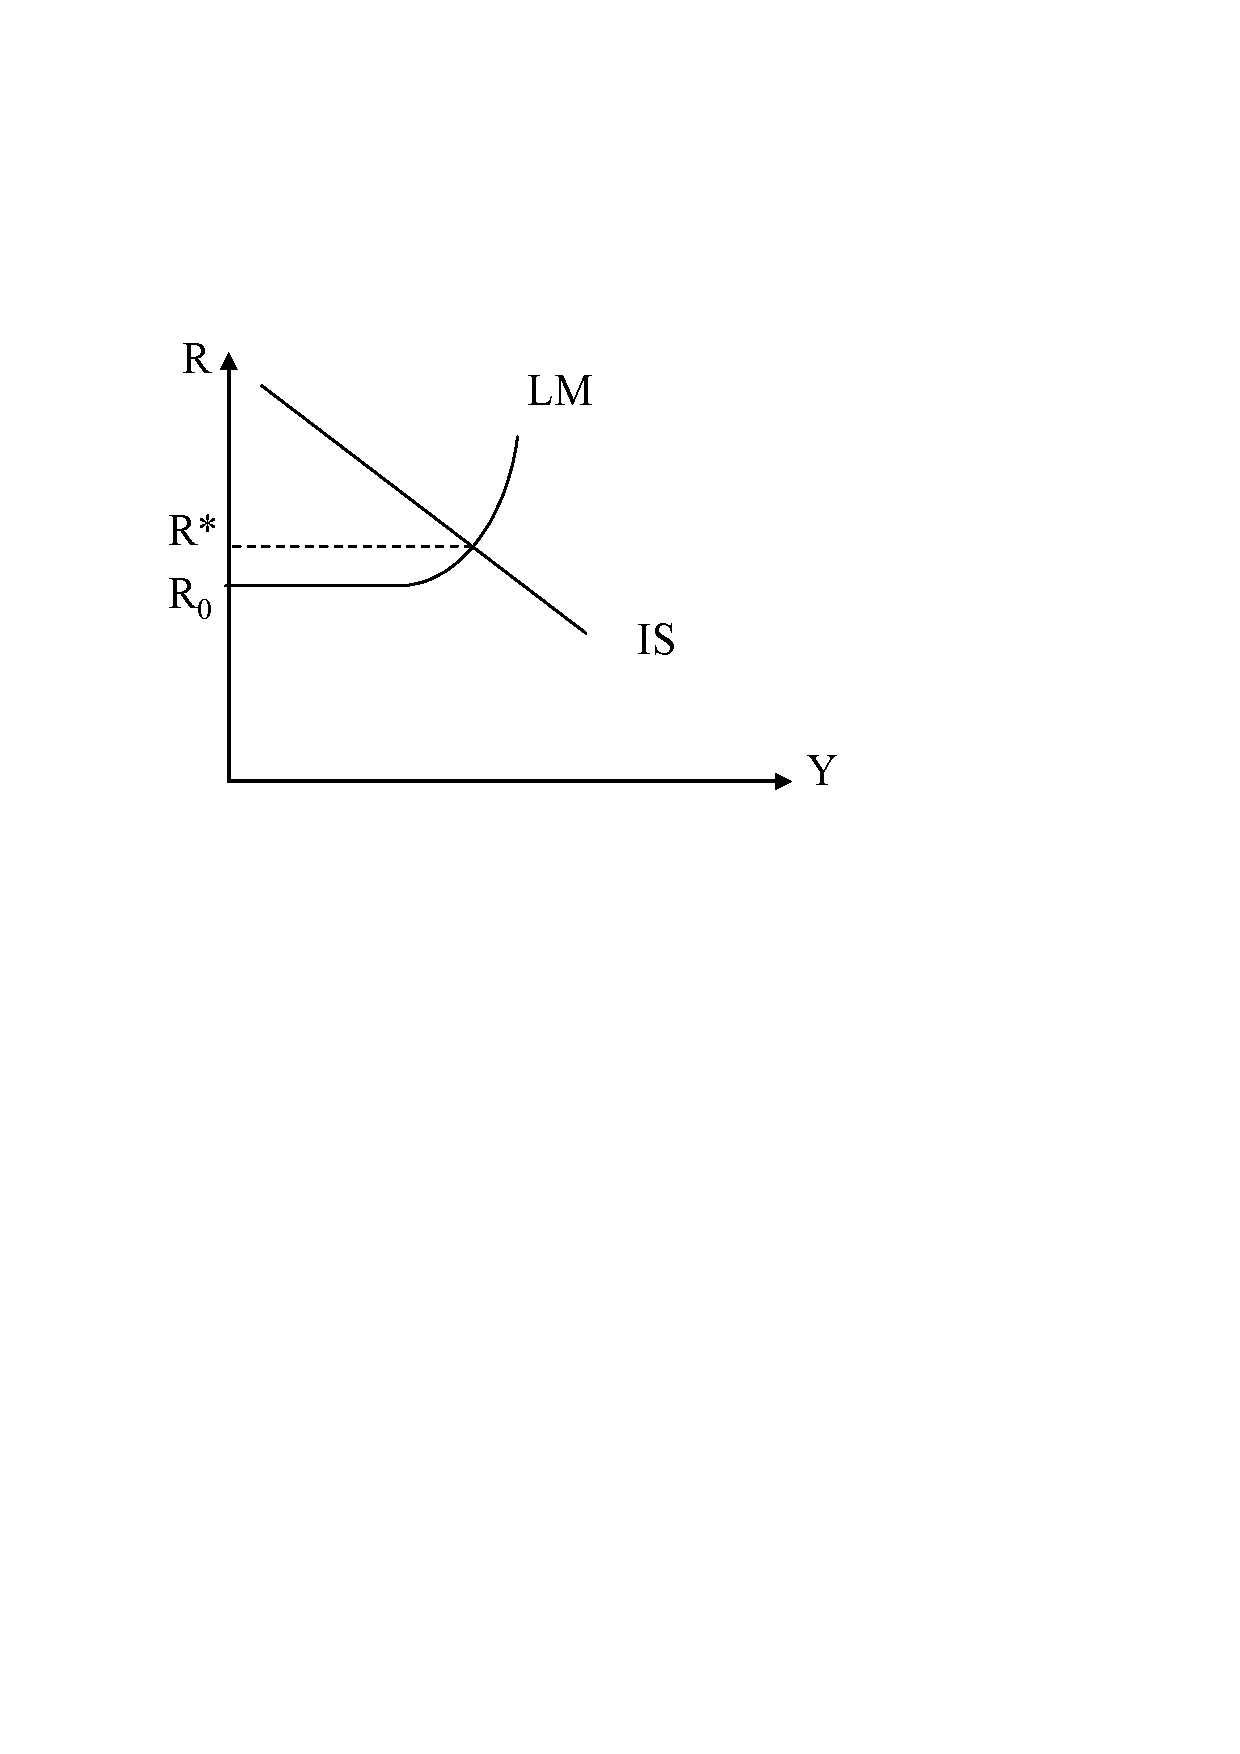
\includegraphics[width=0.5\textwidth]{Bilder/ISLM2.pdf}\end{center}
\begin{enumerate}
	\item Eine stetige Erhöhung der Geldmenge würde die LM-Kurve schrittweise so weit nach rechts verschieben, bis sich der Zinssatz null Prozent annähert (falsch).
	\item Eine Erhöhung der Staatsausgaben, die durch eine entsprechend große Erhöhung der Geldmenge finanziert wird, führt nur zu einer parallelen Rechtsverschiebung der Kurven um den gleichen Betrag und hat daher keinen Effekt auf das Einkommen. (falsch)
	\item Eine stetige Senkung von Staatsausgaben und autonomen Investitionen kann den Zins nicht unter $R_0$ drücken. (wahr)
	\item Sowohl eine starke Erhöhung der Geldmenge als auch eine starke Senkung der Staatsausgaben könnte die dargestellte Volkswirtschaft in die Situation einer Liquiditätsfalle bringen, obwohl sich die Volkswirtschaft in der Ausgangssituation nicht in der Liquiditätsfalle befindet. (wahr)
	\item Eine Geldmengenerhöhung verschiebt die LM-Kurve nach rechts, nicht nach rechts unten. Daher kann der minimale Zinssatz, bei dem die Liquiditätsfalle einsetzt, durch Geldpolitik nicht verändert werden. (wahr)
	\item Die Keynesianische Idee eines Unterbeschäftigungsgleichgewichts besagt, dass sich ein stabiles Gleichgewicht auch abseits des Schnittpunktes von IS- und LM-Kurve halten kann. (falsch)
\end{enumerate}

\subsection{Klassischer Verlauf der LM Kurve}
Betrachten sie die Keynesianische Modellwelt. Die Zinsreagibilität der Geldnachfrage betrage 0.
\begin{enumerate}
	\item Skizzieren sie zunächst die Situation in einem i-Y-$L_T$-$L_s$ 4-Quadranten-Diagramm.
	\item Die Staatsausgaben mögen nun steigen. Zeigen sie in ihrem Diagramm, welche Auswirkungen dies auf den Zins, das Volkseinkommen, die Transaktions- und die Spekulationskasse hat. Wie ändern sich Investitionen und die Ersparnis?
\end{enumerate}



\subsection{Investitionsfalle im IS-LM Modell}
Betrachten sie die Keynesianische Modellwelt. Die Zinsreagibilität der Investitionen betrage 0.
\begin{enumerate}
	\item Skizzieren sie zunächst die Situation in einem i-Y-S-I 4-Quadranten-Diagramm.
	\item Die autonomen Investitionen mögen nun einmalig sinken. Zeigen sie in ihrem Diagramm, welche Auswirkungen dies auf den Zins, die Investitionen, die Ersparnis und das Volkseinkommen hat. Begründen sie auch den Einfluss auf die Spekulations- und Transaktionskasse.
\end{enumerate}

\subsection{Rechenaufgabe}
Eine geschlossene Volkswirtschaft mit staatlicher Aktivit\"{a}t wird durch
folgendes Modell beschrieben:
\begin{align*}
    &\text{Konsumfunktion: } &\quad& C = 10 + 0.5\cdot (Y-T)\\
    &\text{Investitionsfunktion: } &\quad&I = 50-40\cdot i\\
    &\text{Staatsausgaben: } &\quad& G=20\\
    &\text{Steuereinnahmen: } &\quad& T=20 + 0.6\cdot Y\\
    &\text{Gesamtwirtschaftliche Nachfrage: } &\quad&Z = C + I + G\\
    &\text{Gleichgewichtsbedingung: } &\quad&Z = Y^s\\
    &\text{G\"{u}terproduktion gleich Volkseinkommen: } &\quad& Y^s = Y
\end{align*}
L\"{o}hne und Preise sind fix, wobei $P=1$. Nehmen Sie f\"{u}r die Teilaufgaben (a)
und (b) an, dass der Zins $i$ exogen gegeben ist. Seine H\"{o}he betr\"{a}gt 25\%.
\begin{enumerate}[(a)]
  \item Wie hoch ist das gleichgewichtige Volkseinkommen? %($Y^*=75$)
  \item Wie \"{a}ndern sich das gleichgewichtige Volkseinkommen und die
      gleichgewichtigen Steuereinnahmen, wenn der Staat die autonomen
      Steuern um $d T_0 =8$ erh\"{o}ht? %$(dY^*=\frac{-5}{8}\cdot dT^a=\frac{-5}{8}\cdot 8 = -5$ und $dT^* = dT^a + 0.6\cdot dY^* = 8 +0.6\cdot(-5) = 5)$
\end{enumerate}
Gehen Sie nun wieder von den urspr\"{u}nglichen Gleichungen aus.
      Dar\"{u}ber hinaus charakterisieren die folgenden Gleichungen die
      betrachtete Volkswirtschaft:
\begin{align*}
  &\text{Reales Geldangebot: } &\quad& \frac{M}{P}=11.5\\
  &\text{Reale Geldnachfrage: } &\quad& L= 0.2\cdot Y - 30\cdot i
\end{align*}
Zus\"{a}tzlich ist der Zins nun eine \emph{endogene} Gr\"{o}{\ss}e.
\begin{enumerate}[(c)]
  \item Wie hoch ist der gleichgewichtige Konsum der Haushalte? %$(C^* = 16)$
\end{enumerate}

\subsection{Verst\"{a}ndnisfragen (wahr/falsch)}
Betrachten Sie die Graphik des folgenden IS-LM-Modells und nehmen Sie
Stellung zu den Aussagen!\\
\begin{center}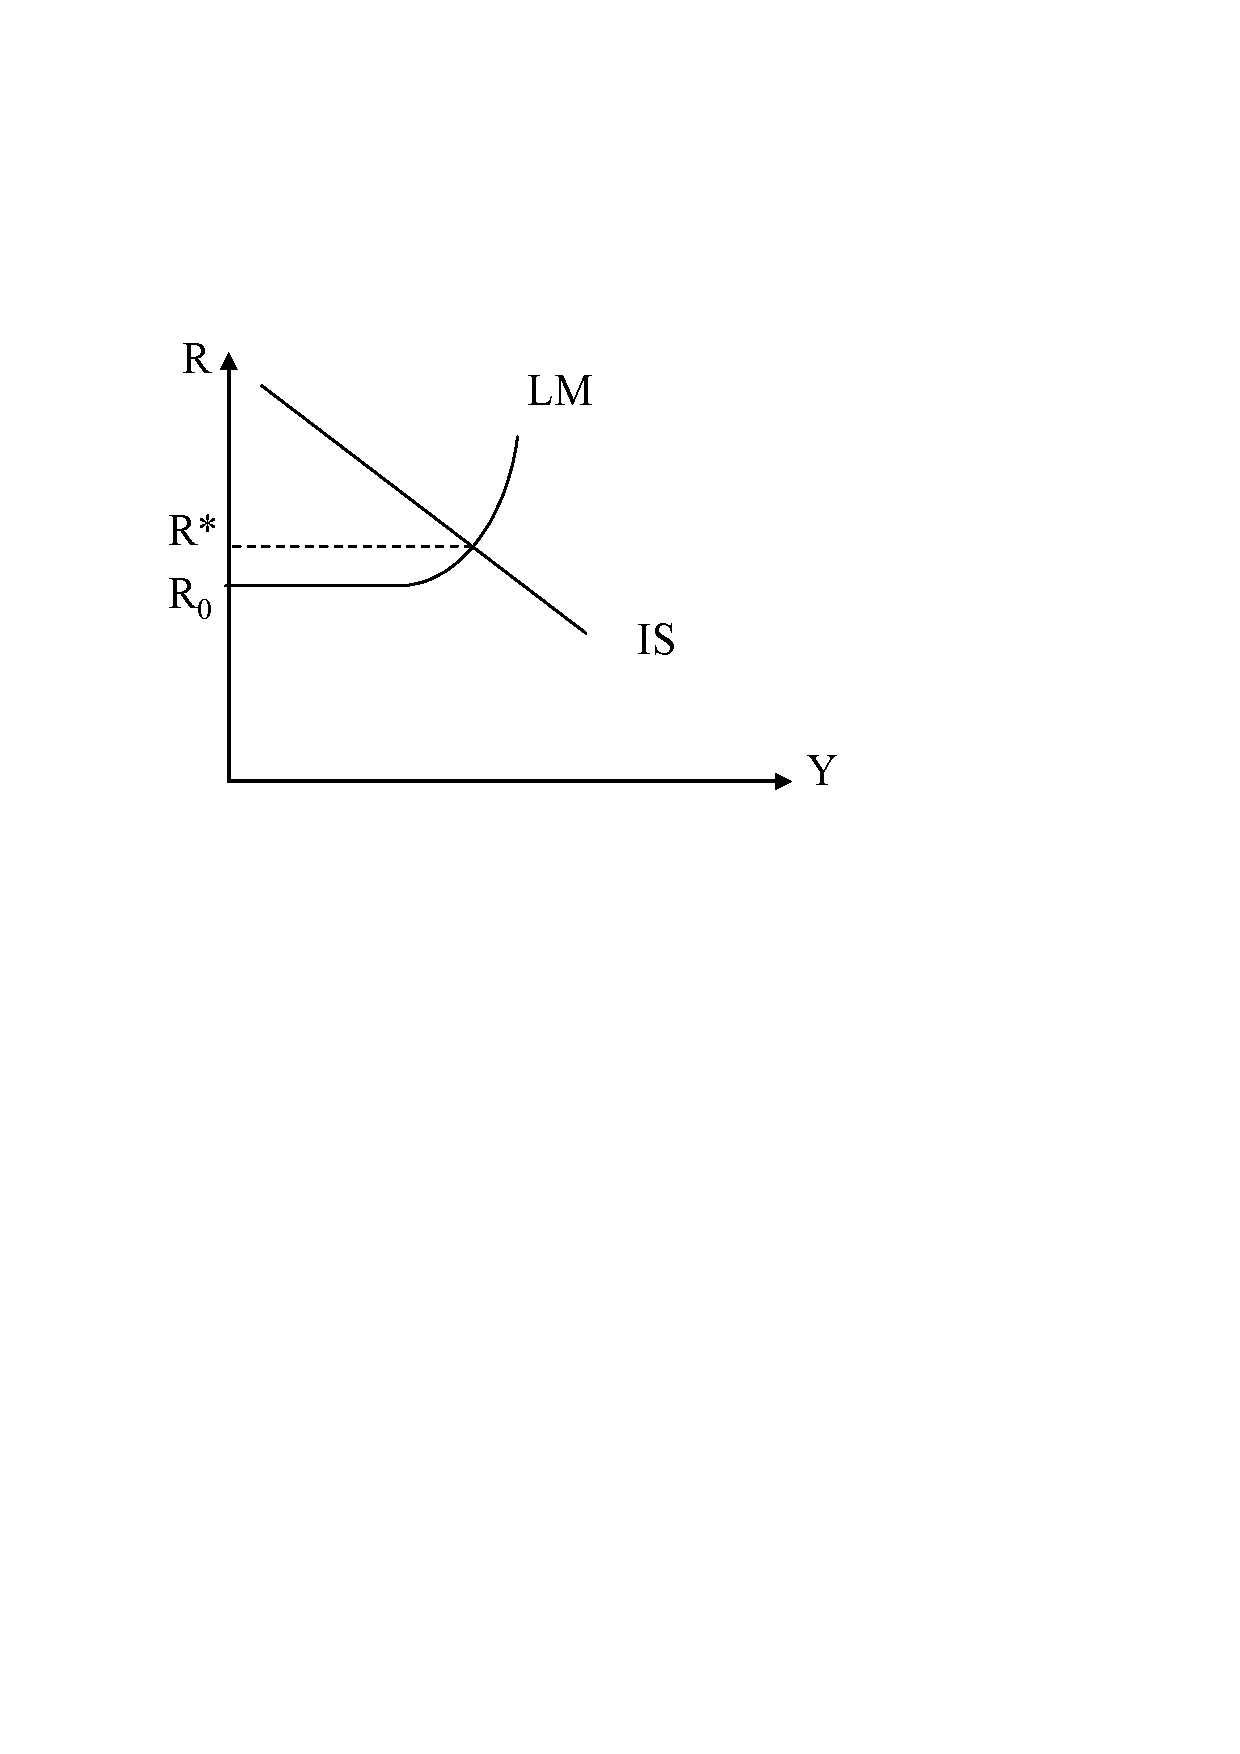
\includegraphics[width=0.5\textwidth]{Bilder/ISLM2.pdf}\end{center}
\begin{enumerate}
  \item Eine Erh\"{o}hung der Staatsausgaben, die durch eine entsprechend
      gro{\ss}e Erh\"{o}hung der Geldmenge finanziert wird, f\"{u}hrt nur zu einer
      parallelen Rechtsverschiebung der Kurven um den gleichen Betrag und
      hat daher keinen Effekt auf das Einkommen. %(falsch)
  \item Eine stetige Senkung von Staatsausgaben und autonomen
      Investitionen kann den Zins nicht unter $R_0$ dr\"{u}cken. %(wahr)
  \item Sowohl eine starke Erh\"{o}hung der Geldmenge als auch eine starke
      Senkung der Staatsausgaben k\"{o}nnte die dargestellte Volkswirtschaft
      in die Situation einer Liquidit\"{a}tsfalle bringen, obwohl sich die
      Volkswirtschaft in der Ausgangssituation nicht in der
      Liquidit\"{a}tsfalle befindet. %(wahr)
  \item Eine Geldmengenerh\"{o}hung verschiebt die LM-Kurve nach rechts,
      nicht nach rechts unten. Daher kann der minimale Zinssatz, bei dem
      die Liquidit\"{a}tsfalle einsetzt, durch Geldpolitik nicht ver\"{a}ndert
      werden. %(wahr)
\end{enumerate}
Gehen sie nun davon aus, dass in einer \"{O}konomie $C=c_0+c_1 Y, I=I(r)$, $M^d=P Y L(r)$ gelte. Die nominale Geldmenge sei $M$ und die Staatsausgaben $G$. Dann gilt dass bei \textbf{einem klassischen Verlauf der Geldnachfrage}
\begin{enumerate}
  \item[5.] expansive Fiskalpolitk zu vollst\"{a}ndigem Crowding-Out der Investitionen f\"{u}hrt.% (wahr)
\item[6.] der Outputeffekt expansiver Geldpolitik kleiner ist als bei einer zinsabh\"{a}ngigen Geldnachfrage. % (falsch)
\end{enumerate}

\subsection{Verständnisfragen Keynesianische Theorie (wahr/falsch)}
\begin{enumerate}
	\item Die Idee der effektiven Nachfrage, die das Say'sche Theorem faktisch umkehrt, reicht für sich allein genommen nicht aus, um Unterbeschäftigungsgleichgewichte zu begründen. (wahr)
	\item Die Idee der effektiven Nachfrage, die das Say’sche Theorem faktisch umkehrt, zwingt jede Ökonomie im Keynesianischen Modell in ein Unterbeschäftigungsgleichgewicht. (falsch)
	\item Der keynesianische Gleichgewichtsbegriff beschreibt die planmäßige Räumung aller Märkte. (falsch)
	\item Keynes fundamentales psychologisches Gesetz, das die Grundlage seiner Konsumfunktion darstellt, beschreibt nichts anderes als abnehmenden Grenznutzen von Konsum. (falsch)
	\item Der keynesianische Multiplikator beruht darauf, dass höherer Konsum die Erwartungen der Investoren verbessert und so zu mehr Investitionen beiträgt. (falsch)
	\item Der Multiplikator ist um so kleiner, je mehr Effekte die Einkommenswirksamkeit der zusätzlichen Nachfrage schmälern. (wahr)
	\item Bei Markträumung (also im Gleichgewicht) ist es möglich, dass die Gesamtnachfrage das Gesamtangebot übersteigt, so das ein Wirtschaftssubjekt nur weniger als die von ihm zum herrschenden Preis gewünschte Gütermenge nachfragen kann. (falsch)
	\item Streng genommen bildet die IS-Kurve kein Kapitalmarktgleichgewicht ab, sondern vielmehr ein Gütermarktgleichgewicht. (falsch)
	\item Die Senkung der Pauschalsteuer hat die gleichen Multiplikatoreffekte, wie eine Ausdehnung der Staatsausgaben um den gleichen Betrag, da die effektive Nachfrage im gleichen Maße gesteigert wird. (falsch)
	\item In der Liquiditätsfalle ist die Geldnachfrage unendlich Zinselastisch. (wahr)
	\item Der Wertpapiermarkt ist im Keynesianischen Modell das Spiegelbild des Geldmarktes. Überschussnachfragen auf dem Geldmarkt bedeutet daher Überschussangebot auf dem Wertpapiermarkt. (wahr)
\end{enumerate}
\newpage

\section{Lundberg und Robertson Lag}
\subsection{Verständnisfragen}
\begin{enumerate}
	\item Unterscheiden Sie das Lundberg-Lag vom Robertson-Lag. Welche grundsätzlichen Implikationen weisen die beiden Lags im Zusammenhang mit der Keynesianischen Theorie auf?
	\item Betrachten Sie nun ein einfaches Keynesianisches Grundmodell
	\begin{align*}
	C  = C_{aut} + c Y, \qquad I  = I_{aut}, \qquad G = G_{aut}
	\end{align*}
	\begin{enumerate}
		\item Berechnen Sie das gleichgewichtige Einkommen $Y^*$ für
		$$ C_{aut} = 50, \qquad I_{aut}=50, \qquad G_{aut}=100, \qquad c=0.5$$
		\item Wie verhält es sich hier mit dem Lundberg-Lag und dem Robertson-Lag? Interpretieren Sie dies auch ökonomisch.
		\item Gehen nun davon aus, dass die Ökonomie sich in Periode t im Gleichgewicht befindet. Die Regierung beschließt in Periode $t+1$ die Staatsausgaben \textbf{permanent} auf $G_{aut}=150$ anzuheben. Zeigen Sie sowohl für das Lundberg-Lag als auch für das Robertson-Lag die Auswirkungen im Zeitverlauf. Nutzen Sie hierfür Sequenztabellen.
	\end{enumerate}
\end{enumerate}

\subsection{Rechenaufgabe Robertson Lag}
In einer geschlossenen Volkswirtschaft mit Staat liegt dem Konsumverhalten der Haushalte ein Robertson-lag zugrunde. Gegeben seien folgende Variablen in der Gleichgewichtsperiode t=0:
\begin{itemize}
	\item Marginale Konsumquote: $c = 0,75$
	\item Autonomer Konsum: $C_{aut} = 0$
	\item Autonome Investitionen: $I_{aut} = 10$
	\item Staatsausgaben (kreditfinanziert): $G = 25$
\end{itemize}
In Periode $t=1$ steigen die autonomen Investitionen dauerhaft auf $I_{aut} = 30$. Vervollständigen Sie die untenstehende Sequenztabelle und berücksichtigen Sie auch geplante und ungeplante Ersparnisse.\\
\begin{center}
	\begin{tabular}{|l|l|l|l|l|l|}
		\hline
		Periode      & 0   & 1   & 2   & ... & $\infty$ \\ \hline
		$Y_{t-1}$    & 140 & 140 & 160 & ... &          \\ \hline
		$C_t$          & 105 & 105 &     & ... &          \\ \hline
		$I_{t}$    & 10  & 30  & 30  & ... & 30       \\ \hline
		$G_t$          & 25  & 25  & 25  & ... & 25       \\ \hline
		$Y_t$        & 140 & 160 &     & ... &          \\ \hline
		$S_{gepl,t}$   & 35  &     &     & ... &          \\ \hline
		$S_{ungepl,t}$ & 0   &     &     & ... & 0        \\ \hline
	\end{tabular}
\end{center}

\subsection{Rechenaufgabe Lundberg Lag}
In einer geschlossenen Volkswirtschaft mit Staat liegt dem Konsumverhalten der Haushalte ein Lundberg-lag zugrunde. Gegeben seien folgende Variablen in der Gleichgewichtsperiode t=0:
\begin{itemize}
	\item Marginale Konsumquote: $c = 0,8$
	\item Autonomer Konsum: $C_{aut} = 0$
	\item Autonome Investitionen: $I_{aut} = 30$
	\item Staatsausgaben (kreditfinanziert): $G = 0$
\end{itemize}
In Periode $t=1$ steigen die Staatsausgaben dauerhaft auf $G = 10$. Vervollständigen Sie die untenstehende Sequenztabelle und berücksichtigen Sie auch ungeplante Investitionen.\\
\begin{center}
	\begin{tabular}{|l|l|l|l|l|l|}
		\hline
		Periode        & 0   & 1   & 2   & ... & $\infty$ \\ \hline
		$Y_{t}$        & 150 & 150 &     & ... &          \\ \hline
		$C_t$          & 120 & 120 &     & ... &          \\ \hline
		$I_{t}$        & 30  & 30  & 30  & ... & 30       \\ \hline
		$G_t$          & 0   & 10  & 10  & ... & 10       \\ \hline
		$S_t$          & 30  &     &     & ... &          \\ \hline
		$I_{ungepl,t}$ & 0   &     &     & ... & 0        \\ \hline
	\end{tabular}
\end{center}

\newpage
\section{Hick'sche Wachstumsmodell}

\subsection{Verständnisfragen}
Betrachten Sie folgendes Multiplikator-Akzelerator Modell nach Hicks:
\begin{align*}
C_t &= C_{aut} + c Y_{t-1}\\
I_t &= I_{aut} + a\cdot (Y_{t-1}-Y_{t-2})\\
Y_t &= C_t + I_t + G_t
\end{align*}
\begin{enumerate}
	\item Erläutern und beschreiben Sie die Gleichungen. Gehen Sie hier insbesondere auf die Rolle von Investitionen und dem Kapitalstock ein.
	\item Warum wird a als Akzelerator bezeichnet?
	\item Gehen Sie nun von folgendem Zahlenbeispiel für die Ökonomie aus:
	\begin{align*}
	G_{aut} = 100, \qquad I_{aut}=50, \qquad C_{aut}=50, \qquad c= 0.5, \qquad a =1
	\end{align*}
	\begin{enumerate}
		\item Berechnen Sie zunächst das stabile Einkommen für dieses Zahlenbeispiel.
		\item Nehmen Sie nun ein stabiles Einkommen in Periode t an und zeigen Sie, wie sich eine \textbf{einmalige} Erhöhung der Staatsausgaben um 50 in Periode $t+4$ auf Konsum, Investitionen, Staatsausgaben und das Volkseinkommen auswirkt. Nutzen Sie hierfür eine Sequenztabelle.
		\item Welche Implikationen hätten andere Werte des Akzelerators?
	\end{enumerate}
\end{enumerate}

\subsection{Rechenaufgabe}
Für ein Hicks'sche Konjunkturmodell gelten folgende Annahmen:
\begin{multicols}{2}
	\begin{itemize}
		\item Marginale Konsumquote: $c = 0,8$
		\item Autonomer Konsum: $C_{aut} = 50$
		\item Autonome Investitionen: $I_{aut} = 140$
		\item Staatsausgaben in $t=0$: $G = 20$
		\item Staatsausgaben in $t=1$: $G = 40$
		\item Akzelerator: a=0,9
	\end{itemize}
\end{multicols}
\begin{enumerate}
	\item Vervollständigen Sie auf Basis des Multiplikator-Akzelerator-Modells von Hicks die abgebildete Sequenztabelle:
	\begin{center}
		\begin{tabular}{|l|l|l|l|l|l|}
			\hline
			Periode      & 0    & 1    & 2    & 3 \\ \hline
			$C$          & 890  & 890  & 906  & 933,20          \\ \hline
			$I_{ind}$    & 0    & 0    &      & 30,60       \\ \hline
			$G$          & 20   & 40   & 40   & 40       \\ \hline
			$Y$          & 1050 & 1070 & 1104 &           \\ \hline
		\end{tabular}
	\end{center}
	\item Wie hoch ist das neue Gleichgewichtseinkommen?
	\item Welche Stabilitäts- und Schwingungseigenschaften hat das Modell?
	\item Wie hoch wäre das neue Gleichgewichtseinkommen, wenn der Akzelerator den Wert 2 hätte und die Staatsausgaben in Periode $t=1$ von 20 auf 40 steigen würden?
\end{enumerate}

\newpage
\section{Neoklassische Synthese}
\subsection{Aggregierte Nachfrage (AD-Modell)} Folgende
Gleichungen beschreiben eine geschlossene Volkswirtschaft mit
Staatstätigkeit:
\begin{align*}
&\text{IS-Kurve: }& Y &= C_{aut} + I_{aut} + G_{aut} + c\cdot (Y-T_{aut}) -b \cdot i\\
&\text{LM-Kurve: }& M_{aut} &= P\cdot L(Y,i) = P\cdot (l \cdot Y - k \cdot i)
\end{align*}
\begin{enumerate}[(a)]
	\item Leiten Sie die aggregierte Nachfragefunktion sowohl graphisch als auch analytisch her. Wie kann diese Funktion interpretiert werden, insbesondere im Hinblick auf eine mikroökonomische Nachfragefunktion? Vergleichen Sie diese Funktion mit der gesamtwirtschaftlichen Güternachfragefunktion im (neo-)klassischen Modell. Machen Sie den Versuch festzustellen, wie die aggregierte Nachfrage im obigen Modell auf Zinssatzänderungen reagiert.
	\item Erklären Sie den Einfluss der autonomen Ausgaben und des autonomen Geldangebots auf die Lage der aggregierten Nachfragekurve.
\end{enumerate}

\subsection{Keynesianisches Totalmodell}
Betrachten Sie nun das Keynesianische Gesamtsystem.
\begin{enumerate}[(a)]
	\item Erklären Sie den Begriff der \enquote{neoklassischen Synthese}. Gehen Sie dabei sowohl auf die Angebots- als auch auf die Nachfrageseite ein und erklären Sie den Keynes-Effekt. Zeigen Sie auch die Wirkung von Fiskal- und Geldpolitik in einem Diagramm.
	\item Wann kommt es zu einem Gleichgewicht (im Sinne einer in sich beharrenden Situation) bei Unterbeschäftigung? Gehen Sie dabei auf die Beschäftigung, das Einkommen, den Zinssatz, das Preisniveau, den Konsum und die Investitionen ein.
	\item Gehen Sie von einem Gleichgewicht bei Unterbeschäftigung aus. Lässt sich mithilfe einer Deflation (also dem Absenken von Preisen, Nominallöhnen und Zinsen) das (neoklassische) Gleichgewicht bei Vollbeschäftigung erreichen? Diskutieren Sie hierbei die Wirkungskanäle von Fiskal- und Geldpolitik.
	\item Zeigen Sie graphisch die Situation
	\begin{enumerate}[(i)]
		\item in einer Investitionsfalle,
		\item in einer Liquiditätsfalle,
		\item bei starren Nominallöhnen
	\end{enumerate}
	und diskutieren Sie die Wirkung von Fiskal- und Geldpolitik mittels einer geeigneten Grafik.
\end{enumerate}

\subsection{Demografische Entwicklung in der neoklassischen Synthese}
Gehen Sie von der Modellwelt der neoklassischen Synthese bei flexiblen Preisen und Nominallöhnen aus. Nehmen Sie nun an, das Arbeitsangebot gehe aus demografischen Gründen zurück. Analysieren Sie anhand einer Grafik, welche Auswirkungen dies auf das Gleichgewicht der Ökonomie hat. Erläutern Sie den Anpassungsprozess vom alten zum neuen Gleichgewicht anhand einer Wirkungskette.

\subsection{Wirtschaftspolitische Maßnahmen in der neoklassischen Synthese}
Betrachten sie die Modellwelt der neoklassischen Synthese. Der Gütermarkt sei geräumt. Untersuchen sie nun die Auswirkungen auf das Arbeitsangebot, die Arbeitsnachfrage, das Realeinkommen, das Preisniveau, das Zinsniveau und den Reallohn in folgenden Situationen:
\begin{enumerate}[(a)]
	\item Die staatlichen Ausgaben für Güter steigen maßvoll an. Nehmen sie flexible Nominallöhne an.
	\item Die staatlichen Ausgaben für Güter sinken maßvoll. Nehmen sie starre Nominallöhne an.
	\item Die Zentralbank erhöht die Geldmenge. Nehmen sie flexible Nominallöhne an.
	\item Die Zentralbank senkt die Geldmenge. Nehmen sie starre Nominallöhne an.
\end{enumerate}




\newpage
\section{Geldtheorie}
\subsection{Rechenaufgabe}
Nehmen Sie an, dass der Anteil des Bargeldes an der Geldmenge 15\% beträgt und der
Mindestreservesatz 0.02 ist. Berechnen Sie den Geldschöpfungsmultiplikator. %5.98\%

\subsection{Verständnisfragen (wahr/falsch)}
\begin{enumerate}
	\item Halten Geschäftsbanken immer Überschußreserven, wird in einer Volkswirtschaft das maximale Geldschöpfungspotential nicht ausgeschöpft, weil immer noch Giralgeld geschaffen werden könnte. (wahr)
	\item Wenn der Mindestreservesatz steigt, dann sinkt bei gegebener Barabhebungsquote immer das Geldschöpfungspotential. (wahr)
	\item Das Aufstellen neuer EC-Automaten senkt ceteris paribus die durchschnittliche Bargeldhaltung, da die realen Transaktionskosten abnehmen. (wahr)
	\item Bei einer Offenmarktpolitik der Zentralbank (Kauf von Wertpapieren) ist die maximale Änderung der Geldmenge nicht abhängig davon, ob die Wertpapiere im Besitz einer
	Geschäftsbank oder eines Unternehmens waren. (wahr)
	\item Wollen die Nichtbanken einen höheren Bargeldanteil halten, steigt ceteris paribus die maximale Kreditvergabemöglichkeit der Banken. (falsch)
	\item Wenn es keine Überschussreserven gibt, dann sinkt der Geldmultiplikator, wenn der Mindestreservesatz steigt. (wahr)
	\item Bei der Geldschöpfung durch Geschäftsbanken wird immer Giralgeld geschaffen. (wahr)
	\item Die Annahme, dass die Geldmenge exogen vorgegeben ist, bedeutet, dass die Zentralbank sie nicht steuern kann. (falsch)
	\item Keynes unterscheidet in der Geldhaltung Vorsichtsmotiv, Transaktionsmotiv und Spekulationsmotiv. (wahr)
	\item Die wesentlichen Geldfunktionen sind Recheneinheit, Tauschmittel und Homogenität. (falsch)
\end{enumerate}


\subsection{Klausuraufgaben}
\begin{enumerate}
  \item Analysieren Sie im Rahmen des IS-LM-Modells die Auswirkungen einer expansiven Fiskalpolitik. Nutzen Sie daf\"{u}r eine geeignete Grafik und stellen Sie die Zusammenh\"{a}nge anhand einer Wirkungskette dar.
  \item Analysieren Sie die Auswirkungen einer Erh\"{o}hung der Geldmenge auf das Inlandseinkommen und den Inlandszins im Rahmen des IS-LM-Modells anhand einer Wirkungskette und einer geeigneten Grafik.
  \item Die \"{O}konomie befinde sich nun in einer Investitionsfalle. Charakterisieren Sie ein solches Szenario zun\"{a}chst verbal, und erl\"{a}utern Sie dann anhand einer Grafik und mittels einer Wirkungskette, wie sich das Ergebnis aus Teilaufgaben (1) und (2) in diesem Fall ver\"{a}ndert.
  \item Die \"{O}konomie befinde sich nun in einer Liquidit\"{a}tsfalle. Charakterisieren Sie ein solches Szenario zun\"{a}chst verbal, und erl\"{a}utern Sie dann anhand einer Grafik und mittels einer Wirkungskette, wie sich das Ergebnis aus Teilaufgaben (1) und (2) in diesem Fall ver\"{a}ndert.
  \item Diskutieren Sie die Wirkungen einer Steuersenkung grafisch und verbal im IS-LM-Modell. Identifizieren Sie in der Grafik die Multiplikatorwirkung, und begründen Sie,  warum sich der Multiplikator im IS-LM-Modell von jenem des Gütermarktmodells
  unterscheidet. Wie ändert sich ihr Ergebnis im Fall einer Liquiditätsfalle?
\end{enumerate}

\newpage
\section{Offene Volkswirtschaft und Mundell-Fleming}

\subsection{Offene Volkswirtschaft}
\begin{enumerate}[(a)]
\item Welche Annahmen liegen dem Modell einer offenen Volkswirtschaft zugrunde? Erkl\"{a}ren Sie dabei die Begriffe Zahlungsbilanz, Wechselkurs und Devisenmarkt.
\item Wie gro{\ss} ist die gesamtwirtschaftliche Ersparnis im Gleichgewicht? Beschreiben Sie den Zusammenhang zwischen internationalen Kapitalbewegungen und dem internationalen Handel.
\end{enumerate}
\subsection{Mundell-Fleming}
Betrachten Sie folgendes Modell einer offenen Volkswirtschaft:
\begin{align}
  Y = C(Y)+I(i)+G+X(Y^*,S)-IM(Y,S)\\
  D + R = L(Y,i)\\
  X(Y^*,S)-IM(Y,S)+F(i,i^*)=0
\end{align}
\begin{enumerate}[(a)]
  \item Definieren und erl\"{a}utern Sie die einzelnen Gleichungen, gehen Sie dabei insbesondere auf die ZZ-Kurve ein. Stellen Sie das Modell graphisch in einem IS-LM-Schema dar und erl\"{a}utern Sie, wodurch die Lage und Verlauf der ZZ-Kurve bestimmt wird. Charakterisieren Sie die Bedeutung von Punkten oberhalb sowie unterhalb der ZZ-Kurve.
  \item Gehen Sie von fixen Wechselkursen aus. Vergleichen Sie anhand geeigneter Grafiken die Auswirkungen von expansiver Geld- und Fiskalpolitik bei hoher Kapitalmobilit\"{a}t. Erl\"{a}utern Sie auch die Wirkungsketten und die \"{o}konomischen Zusammenh\"{a}nge.
  \item Gehen Sie von flexiblen Wechselkursen aus. Vergleichen Sie anhand geeigneter Grafiken die Auswirkungen von expansiver Geld- und Fiskalpolitik bei hoher Kapitalmobilit\"{a}t. Erl\"{a}utern Sie auch die Wirkungsketten und die \"{o}konomischen Zusammenh\"{a}nge.
  \item Gehen Sie nun von perfekter Kapitalmobilit\"{a}t und flexiblen Wechselkursen aus. Vergleichen Sie anhand geeigneter Grafiken die Auswirkungen von expansiver Geld- und Fiskalpolitik. Erl\"{a}utern Sie auch die Wirkungsketten und die \"{o}konomischen Zusammenh\"{a}nge.
  \item Untersuchen Sie bei perfekter Kapitalmobilit\"{a}t den Einfluss des ausl\"{a}ndischen Konjunkturzyklus auf die \"{O}konomie bei festen und flexiblen Wechselkursen.
\end{enumerate}

\subsection{Klausuraufgaben}
Betrachten Sie eine offene Volkswirtschaft in der kurzen Frist, die durch folgendes Gleichungssystem beschrieben werden kann:
\begin{align*}
  Y = C(Y)+I(i)+G +X(Y^*,S)-IM(Y,S)\\
  D+R = L(Y,i)\\
  X(Y^*,S) - IM(Y,S)+F(i,i^*)=0
\end{align*}
\begin{enumerate}
  \item Betrachten Sie das Modell mit hoher Kapitalmobilit\"{a}t. Analysieren Sie die Wirkungen einer Geldmengenerh\"{o}hung bei flexiblen Wechselkursen im Fall einer Investitionsfalle mittels einer Wirkungskette und anhand einer geeigneten Grafik.
  \item Skizzieren Sie die Bedingung f\"{u}r ein Zahlungsbilanz- und Devisenmarktgleichgewicht anhand der dritten Gleichung, zeichnen Sie die Gleichgewichtsbedingung in ein Zins-Einkommensdiagramm ein, und erl\"{a}utern Sie deren Steigung.
  \item Analysieren Sie die Wirkungen einer Staatsausgabenerh\"{o}hung bei flexiblen Wechselkursen und niedriger Kapitalmobilit\"{a}t in einer offenen Volkswirtschaft mittels einer Wirkungskette und anhand einer geeigneten Grafik.
  \item Analysieren Sie die Wirkungen einer Staatsausgabenerh\"{o}hung bei flexiblen Wechselkursen und niedriger Kapitalmobilit\"{a}t in einer offenen Volkswirtschaft, die sich in der Liquidit\"{a}tsfalle befindet, mittels einer Wirkungskette und anhand einer geeigneten Grafik.
  \item Analysieren Sie die Wirkungen einer Staatsausgabenerh\"{o}hung im Mundell-Fleming-Modell einer kleinen offenen Volkswirtschaft, die keinerlei Finanzbeziehungen zum Rest der Welt unterh\"{a}lt (Szenario ohne jegliche Kapitalmobilit\"{a}t).
\end{enumerate}
\newpage
\section{Arbeitsmarkt und AS-AD Modell}

\subsection{Arbeitsmarkt und Aggregierte Angebot}
Gehen Sie von folgenden Gleichungen als Beschreibung von Firmen- und Arbeitnehmerverhalten einer Volkswirtschaft aus:
\begin{align}
  &\text{Produktionsfunktion: }& Y &= AN\\
  &\text{Preissetzung: }& P &= (1+\mu)W\\
  &\text{Lohnsetzung: }& W &=P^e F(u,z)=P^e z[(1-u)L^s]
\end{align}
wobei A die Arbeitsproduktivit\"{a}t, $N$ die Besch\"{a}ftigung, $u$ die Arbeitslosenquote und $L^s$ das Arbeitsangebot bezeichnen. In $z$ sind weitere Einflussfaktoren des Lohnsatzes $W$ zusammengefasst $(\partial F/\partial z >0)$.
\begin{enumerate}[(a)]
\item Erl\"{a}utern Sie sowohl die Preissetzungs- als auch Lohnsetzungsgleichung.
\item Zeigen Sie den Zusammenhang zwischen Arbeitsangebot, Arbeitslosenquote und Besch\"{a}ftigung. Gehen Sie davon aus, dass die Arbeitnehmer ihre Lohnforderung auf Basis des aktuellen Preisniveuas bilden $(P^e=P)$ und zeichnen Sie die Lohn- und die Preissetzungskurve in ein Diagramm ein, in dem die Besch\"{a}ftigung $N$ auf der Abszisse und der Reallohn $W/P$ auf der Ordinate abgetragen ist. Interpretieren Sie die Darstellung kurz. Zeigen Sie zudem graphisch, welchen Effekt eine Ver\"{a}nderung des Preisaufschlags $\mu$ hat. Geben Sie eine \"{o}konomische Erkl\"{a}rung f\"{u}r eine m\"{o}gliche Ver\"{a}nderung von $\mu$.
\item Ermitteln Sie die AS-Kurve f\"{u}r $A = 1$ und zeigen Sie deren Verlauf qualitativ in einem $(Y,P)$ Diagramm, wenn die Menschen keine korrekten Preiserwartungen bilden $(P^e\neq P)$. Wie wirkt sich eine Erh\"{o}hung des erwarteten Preisniveaus aus?
\item Ermitteln Sie die AS-Kurve f\"{u}r $A = 1$ wenn die Menschen korrekte Preiserwartungen bilden $(P^e=P)$ und zeigen Sie deren Verlauf qualitativ in einem $(Y,P)$ Diagramm. Interpretieren Sie die Darstellung.
\end{enumerate}
\subsection{Aggregierte Nachfrage}
Folgende Gleichungen beschreiben eine geschlossene Volkswirtschaft mit
Staatst\"{a}tigkeit:
\begin{align*}
  &\text{IS-Kurve: }& Y &= C(Y,T) + I(i) + G\\
  &\text{LM-Kurve: }& M &= P L(Y,i)
\end{align*}
\begin{enumerate}[(a)]
  \item Leiten Sie die aggregierte Nachfragefunktion sowohl graphisch als auch analytisch her. Bestimmen Sie auch die Steigung $dP/dY$ formal. Wie kann diese Funktion interpretiert werden, insbesondere im Hinblick auf eine mikro\"{o}konomische Nachfragefunktion?
  \item Machen Sie den Versuch festzustellen, wie die aggregierte Nachfrage im obigen Modell auf Zinssatz\"{a}nderungen reagiert.
  \item Erkl\"{a}ren Sie den Einfluss der autonomen Staatsausgaben und Steuern $(G,T)$ und des autonomen Geldangebots $(M)$ auf die Lage der aggregierten Nachfragekurve.
\end{enumerate}
\subsection{Wirtschaftspolitische Ma{\ss}nahmen im AS-AD Modell}
Nehmen Sie an, eine \"{O}konomie kann durch folgende Zusammenh\"{a}nge beschrieben werden:
\begin{align*}
  C &= 750 + 0,8(Y-T)  &
  I &= -4000 i\\
  G&=T=750 &
  M-P &= 0,2 Y -1000i
\end{align*}
\begin{enumerate}[(a)]
\item Ermitteln Sie die AD-Kurve rechnerisch
\end{enumerate}
Unterstellen Sie im Folgenden zus\"{a}tzlich folgende AS-Kurve:
\begin{align*}
  P = P^e + 0,5(Y-\bar{Y})
\end{align*}
wobei $\bar{Y}$ das Outputniveau bezeichnet, dass sich ergibt, wenn der Arbeitsmarkt im Gleichgewicht ist. Das gleichgewichtige Produktionsniveau sei $\bar{Y}=1200$ und die Geldmenge im Ausgangsgleichgewicht $M_0=600$.
\begin{enumerate}
  \item[(b)] Wie hoch sind das erwartete Preisniveau bei korrekten Erwartungen und der Zinssatz im Gleichgewicht? Stellen Sie das Gleichgewicht auch graphisch dar.
  \item[(c)] Ermitteln Sie rechnerisch unter der Annahme korrekter Erwartungen $(P^e=P)$ Produktion und Preisniveau wenn die nominale Geldmenge auf $M_1 =400$ reduziert wird. Zeigen Sie die Effekte der kontraktiven Geldpolitik auch graphisch.
  \item[(d)] Ermitteln Sie rechnerisch unter der Annahme gegebener Erwartungen $(P_t^e=P_{t-1})$ Produktion und Preisniveau wenn die nominale Geldmenge auf $M_1 =400$ reduziert wird. Zeigen Sie die Effekte der kontraktiven Geldpolitik auch graphisch.
\end{enumerate}

\subsection{Klausuraufgaben}
Betrachten Sie eine Volkswirtschaft in der mittleren Frist. Nehmen Sie an, dass die aggregierte Produktionsfunktion mit $Y = N$ gegeben ist, wobei $N$ die Menge an eingesetzter Arbeit darstellt. Zudem gelten die folgenden Gleichungen:
\begin{align}
  &\text{Preissetzung: }& P &= (1+\mu)W\\
  &\text{Lohnsetzung: }& W &=P^e z[(1-u)L^s]
\end{align}
wobei $u$ die Arbeitslosenquote und $L^s$ die Menge aller Erwerbspersonen bezeichne.
\begin{enumerate}
  \item Beschreiben Sie kurz die Preissetzungs- und die Lohnsetzungsgleichung.
  \item Leiten Sie die AS-Kurve analytisch her und erl\"{a}utern Sie deren Verlauf in der kurzen und mittleren Frist.
  \item Ermitteln Sie aus der hergeleiteten AS-Kurve das nat\"{u}rliche Produktionsniveau sowie die nat\"{u}rliche Arbeitslosenquote.
  \item Unterstellen Sie eine negativ geneigte AD-Kurve, und analysieren Sie grafisch und anhand einer Wirkungskette die Effekte einer kontraktiven Fiskalpolitik auf den Output und das Preisniveau (i) in der kurzen Frist mit konstanten Erwartungen $P^e$ und (ii) in der mittleren Frist mit korrekten Erwartungen $P=P^e$.
    \item Unterstellen Sie eine negativ geneigte AD-Kurve, und analysieren Sie grafisch und anhand einer Wirkungskette die Effekte einer expansiven Geldpolitik auf den Output und das Preisniveau (i) in der kurzen Frist mit konstanten Erwartungen $P^e$ und (ii) in der mittleren Frist mit korrekten Erwartungen $P=P^e$.
    \item Erläutern Sie die kurz- und mittelfristigen Wirkungen einer Steuersenkung im AS-AD-Modell jeweils mit Hilfe einer Grafik und einer Wirkungskette. Vergleichen Sie die Multiplikatorwirkung mit jener im IS-LM-Modell.
    \item Nehmen Sie nun folgende Gleichungen an, wobei $A$ einen Produktivit\"{a}tsparameter darstellt und $A^e$ die Erwartung diesbez\"{u}glich:
    \begin{align}
  &\text{Produktionsfunktion: }& Y &= AN\\
  &\text{Preissetzung: }& P &= (1+\mu)\frac{W}{A}\\
  &\text{Lohnsetzung: }& W &=A^e P^e z[(1-u)L^s]
\end{align}
\begin{enumerate}
\item Leiten Sie die AS-Kurve f\"{u}r gegebene (konstante) Realisationen von $A$, $A^e$ und $P^e$ analytisch her und erl\"{a}utern Sie deren Verlauf.
\item Ermitteln Sie das nat\"{u}rliche Produktionsniveau sowie die nat\"{u}rliche Arbeitslosenquote.
\item Unterstellen Sie eine negativ geneigte AD–Kurve, deren Position nicht vom Produktivit\"{a}tsparameter $A$ abh\"{a}nge. Verwenden Sie ein G\"{u}termarktdiagramm und analysieren Sie rein grafisch (ohne Wirkungskette) die Effekte eines einmaligen Anstiegs des Produktivit\"{a}tsparameters A auf den Output und das Preisniveau (i) in der kurzen Frist mit konstanten Erwartungen $A^e$ und $P^e$ sowie (ii) in der mittleren Frist mit korrekten Erwartungen $A = A^e$ und $P = P^e$. Geben Sie eine kurze verbal-\"{o}konomische Begr\"{u}ndung f\"{u}r ihr Ergebnis.
\end{enumerate}
\end{enumerate}

\section{Phillips-Kurve}
\begin{enumerate}[a)]
  \item Wie lautet der urspr\"{u}ngliche Zusammenhang, den die Phillipskurve zeigt? Welcher \"{o}konomische Mechanismus steht hinter der Beobachtung? Erkl\"{a}ren Sie auch die Lohn-Preis-Spirale.
  \item Leiten Sie die um Erwartungen erweiterte Phillipskurve aus der AS-Kurve ab. Nehmen Sie dazu folgende funktionelle Form an: $F(u,z) = 1-\alpha u +z$.
  \item Inwiefern unterscheidet sich die kurzfristige von der langfristigen Phillips-Kurve? Verdeutlichen Sie dies anhand einer Grafik.
  \item Nehmen Sie nun an, der Zusammenhang zwischen Inflation und Arbeitslosigkeit lasse sich durch folgende Phillipskurve beschreiben:
  \begin{align*}
    \pi_t = \pi_t^e + \alpha(u_n-u)
  \end{align*}
    \begin{enumerate}[(i)]
    \item Interpretieren Sie die Gleichung.
    \item Welche Implikationen haben verschiedene Erwartungsprozesse f\"{u}r den Zusammenhang zwischen Inflation und Arbeitslosigkeit? Inwiefern \"{a}ndert sich der Einfluss von Geldpolitischen Ma{\ss}nahmen in der kurzen Frist?
    \end{enumerate}
Angenommen, die Ökonomie weist eine Arbeitslosigkeit in Höhe von $u_n$, und eine positive Inflation $\pi_t$ auf.
\begin{enumerate}
	\item Die Zentralbank kündigt an, in Zukunft die Inflation schrittweise auf 0 zu senken. Zeigen Sie graphisch, wie sich Inflation und Arbeitslosigkeit im Zeitablauf verändern, wenn die Wirtschaftssubjekte adaptive Erwartungen $\pi_t^e=\pi_{t-1}$ haben.
	\item Angenommen, die Regierung setzt einen neuen Zentralbankchef ein, der für seine strikte Disinflationierungspolitik bekannt ist. Welche Unterschiede könnten sich dadurch zu vorangegangenen Teilaufgabe ergeben?
\end{enumerate}
\end{enumerate}

\section{Solow-Modell}

\subsection{Rechenaufgabe}
Nehmen Sie an, dass die Produktionsfunktion eines Landes gegeben sei durch
\begin{align*}
  Y = AK_t^{0.3}N_t^{0.7}
\end{align*}
Das Verh\"{a}ltnis von Kapital zu Output betrage 3, die Wachstumsrate von Output betrage 3\% und der Abschreibungssatz sei gleich 4\%. Kapital wird durch sein Grenzprodukt entlohnt.
\begin{enumerate}[(a)]
  \item Wie gro{\ss} ist in dieser Situation das Grenzprodukt von Kapital?
  \item Wie gro{\ss} ist die Sparquote s dieser Wirtschaft im langfristigen Gleichgewicht?
  \item Wenn diese \"{O}konomie beschlie{\ss}t, dass sie das Goldene Regel Niveau des Kapitalstocks erreichen m\"{o}chte und dieses Ziel auch verwirklicht, wie gro{\ss} wird dann das Grenzprodukt des Kapitals sein?
  \item Wie gro{\ss} muss die Sparquote $s$ sein, damit die \"{O}konomie das Goldene-Regel Kapitalniveau erreicht?
\end{enumerate}
\subsection{Zwei L\"{a}nder}
Betrachten Sie zwei L\"{a}nder, die sich lediglich darin unterscheiden, dass das Bev\"{o}lkerungswachstum in Land A gr\"{o}{\ss}er ist als das in Land B.
\begin{enumerate}[(a)]
  \item In welchem Land wird die durchschnittliche Arbeitsproduktivit\"{a}t im langfristigen Gleichgewicht h\"{o}her sein? Begr\"{u}nden Sie ihre Antwort graphisch.
  \item In welchem Land wird die Wachstumsrate der durchschnittlichen Arbeitsproduktivit\"{a}t im langfristigen Gleichgewicht h\"{o}her sein? Begr\"{u}ndung?
\end{enumerate}
\subsection{Tropicana}
Es regnet so viel in dem Land Tropicana, dass der Kapitalstock sehr viel schneller verrostet als der Kapitalstock in dem Land Sahara. Unterstellen Sie, dass die beiden L\"{a}nder sonst in jeder Hinsicht identisch sind. In welchem Land wird das Goldene Regel Niveau der Kapitalintensit\"{a}t h\"{o}her sein? Begr\"{u}nden Sie ihre Antwort graphisch.
\subsection{China}
Betrachten Sie China, das 1979 die Ein-Kind Politik f\"{u}r die gesamte Bev\"{o}lkerung verbindlich einf\"{u}hrte. Benutzen Sie das einfache Solow-Modell, um graphisch die Auswirkungen dieser Politik auf das Verh\"{a}ltnis von Kapital zu Arbeit $(K/L)$ und auf die durchschnittliche Arbeitsproduktivit\"{a}t $(Y/L)$ in der langen Frist darzustellen.

\subsection{Solow Konvergenz}
Betrachten Sie das Solow Modell mit einer Cobb-Douglas Produktionsfunktion $Y=K^{\alpha}N^{1-\alpha}$, der Sparquote $s$ und der Bev\"{o}lkerungswachstumsrate $n$.
\begin{enumerate}[(a)]
  \item Leiten Sie einen Ausdruck f\"{u}r die Wachstumsrate des pro-Kopf Kapitalstocks her.
  \item Berechnen Sie, wie die Wachstumsrate aus (a) vom Niveau des pro-Kopf Kapitalstocks abh\"{a}ngt.
  \item Betrachten Sie zwei \"{O}konomien mit unterschiedlichem Kapitalstock $k_1<k_2$. Was bedeutet ihr Ergebnis aus (b) f\"{u}r die Entwicklung der Einkommensverteilung zwischen diesen \"{O}konomien?
  \item Wie \"{a}ndert sich Ihr Ergebnis aus (c), wenn $s_1<s_2$?
\end{enumerate}
\subsection{Klausuraufgaben}
\begin{enumerate}
\item Die Produktionsfunktion einer \"{O}konomie zum Zeitpunkt $t$ lautet $Y_t = AK_t^\alpha N^{1-\alpha}$, wobei $Y_t$ den Output,
$K_t$ den Kapitalstock, $N$ die (konstante) Besch\"{a}ftigung und $A$ einen Produktivit\"{a}tsparameter beschreibt. F\"{u}r den Parameter $\alpha$ gilt $0 < \alpha < 1$. Die Kapitalstockbewegungsgleichung
lautet $K_{t+1} = (1-\delta)K_t + s Y_t$, mit $\delta$ als Abschreibungsrate.
\begin{enumerate}
\item Leiten Sie algebraisch das Steady-State-Gleichgewicht in pro-Kopf-Gr\"{o}{\ss}en her. Von welchen exogenen Einflussfaktoren h\"{a}ngt der gleichgewichtige Pro- Kopf Output ab?
\item Zeichnen Sie das Steady-State-Gleichgewicht in eine geeignete Grafik ein, und analysieren Sie anhand der Grafik die kurz- und langfristigen Auswirkungen
    \begin{enumerate}
    \item einer einmaligen Erh\"{o}hung des Produktivit\"{a}tsparameters $A$
    \item einer verringerten Sparquote
    \item eines Anstiegs der Abschreibungsrate
    \end{enumerate}
    auf die Wachstumsrate dieser \"{O}konomie.
\item Die Kapitalintensit\"{a}t im steady state, $\frac{K^*}{N}$, ist charakterisiert durch $s\left(\frac{K^*}{N}\right)^\alpha = \delta\frac{K^*}{N}$. Erl\"{a}utern Sie diese Gleichung kurz, und leiten Sie aus dieser Gleichung die Bestimmungsgleichung des gleichgewichtigen Pro-Kopf-Outputs her.
\item Stellen Sie in einer geeigneten Grafik die Goldene Regel der Kapitalakkumulation dar. Zeichnen Sie nun ein Steady-State-Gleichgewicht mit einer Kapitalintensit\"{a}t oberhalb der Goldenen Regel ein. Zeigen Sie, ausgehend von diesem Steady-State-Gleichgewicht, wie sich eine Erh\"{o}hung der Sparquote auf die gleichgewichtigen Niveaus des Pro-Kopf-Einkommens und des Pro-Kopf-Konsums auswirkt. Geben Sie eine kurze verbale Erl\"{a}uterung.
\end{enumerate}
\item Eine Volkwirtschaft werde durch ein starkes Erdbeben heimgesucht, welches einen Großteil des Kapitalstocks des Landes vernichtet. Aufgrund eines effektiven Frühwarnsystems fordert
das Erdbeben keine Menschenleben.
\begin{enumerate}
\item Analysieren Sie grafisch und verbal die kurz- und langfristigen Auswirkungen dieser Naturkatastrophe auf Produktion und Wirtschaftswachstum im Solow-Modell. Unterstellen Sie dabei, dass sich die Ökonomie ursprünglich in einem Steady-State-Gleichgewicht befunden hat.
\item Das neu installierte Kapital sei weniger störanfällig, so dass die Abschreibungsrate auf den volkswirtschaftlichen Kapitalstock insgesamt sinkt. Analysieren Sie grafisch und verbal die kurz- und langfristigen Auswirkungen dieser veränderten Abschreibungsrate auf Produktion und Wirtschaftswachstum.
\end{enumerate}
\end{enumerate}

\section{Solow-Modell}

\subsection{Verständnis}
Die Produktionsfunktion einer Ökonomie zum Zeitpunkt $t$ lautet $Y_t=K_t^\alpha N_t^{1-\alpha}$, wobei $Y_t$ den Output, $K_t$ den Kapitalstock und $N_t$ die Beschäftigung beschreibt. Für den Parameter $\alpha$ gilt $0<\alpha<1$. Die Kapitalstockbewegungsgleichung lautet $K_{t+1}=(1-\delta)K_t + s Y_t$, mit $\delta$ als Abschreibungsrate.
\begin{enumerate}[(a)]
\item Leiten Sie algebraisch das Steady-State-Gleichgewicht in pro-Kopf-Größen her. Von welchen exogenen Einflussfaktoren hängt der gleichgewichtige Pro-Kopf Output ab?
\item Zeichnen Sie das Steady-State-Gleichgewicht in eine geeignete Grafik ein, und analysieren Sie anhand der Grafik die kurz- und langfristigen Auswirkungen einer verringerten Sparquote auf die Wachstumsrate dieser Ökonomie.
\end{enumerate}

\subsection{Rechenaufgabe}
Nehmen Sie an, dass die Produktionsfunktion eines Landes gegeben sei durch
\begin{align*}
  Y = A K^{0.3}N^{0.7}
\end{align*}
Das Verhältnis von Kapital zu Output betrage 3, die Wachstumsrate von Output betrage 3\% und der Abschreibungssatz sei gleich 4\%. Kapital wird durch sein Grenzprodukt entlohnt.
\begin{enumerate}[(a)]
  \item Wie groß ist in dieser Situation das Grenzprodukt von Kapital? %($\partial Y/\partial K = 0.3$)
  \item Wie groß ist die Sparquote s dieser Wirtschaft im langfristigen Gleichgewicht? %($s=0.21$)
  \item Wenn diese Ökonomie beschließt, dass sie das Goldene Regel Niveau des Kapitalstocks erreichen möchte und dieses Ziel auch verwirklicht, wie groß wird dann das Grenzprodukt des Kapitals sein? %($f'(k^*)=0.07$)
  \item Wie groß muss die Sparquote $s$ sein, damit die Ökonomie das Goldene-Regel Kapitalniveau erreicht? %($s^*=\alpha=0.4$)
\end{enumerate}


\subsection{Bevölkerungswachstum}
Betrachten Sie zwei Länder, die sich lediglich darin unterscheiden, dass das Bevölkerungswachstum in Land A größer ist als das in Land B.
\begin{enumerate}[(a)]
  \item In welchem Land wird die durchschnittliche Arbeitsproduktivität im langfristigen Gleichgewicht höher sein? Begründen Sie ihre Antwort graphisch.
  \item In welchem Land wird die Wachstumsrate der durchschnittlichen Arbeitsproduktivität im langfristigen Gleichgewicht höher sein?
\end{enumerate}

\subsection{Abschreibungsrate}
Es regnet so viel in dem Land Tropicana, dass der Kapitalstock sehr viel schneller verrostet als der Kapitalstock in dem Land Sahara. Unterstellen Sie, dass die beiden Länder sonst in jeder Hinsicht identisch sind. In welchem Land wird das Goldene Regel Niveau der Kapitalintensität höher sein? Begründen Sie ihre Antwort graphisch.

\subsection{China}
Betrachten Sie China, das 1979 die Ein-Kind Politik für die gesamte Bevölkerung verbindlich einführte. Benutzen Sie das einfache Solow-Modell, um graphisch die Auswirkungen dieser Politik auf das Verhältnis von Kapital zu Beschäftigung $(K/N)$ und auf die durchschnittliche Arbeitsproduktivität $(Y/N)$ in der langen Frist darzustellen.

\subsection{Solow Konvergenz}
Betrachten Sie das Solow Modell mit einer Cobb-Douglas Produktionsfunktion $Y=K^{\alpha}N^{1-\alpha}$, der Sparquote $s$ und der Bevölkerungswachstumsrate $n$.
\begin{enumerate}[(a)]
  \item Leiten Sie einen Ausdruck für die Wachstumsrate des pro-Kopf Kapitalstocks her.
  \item Berechnen Sie, wie die Wachstumsrate aus (a) vom Niveau des pro-Kopf Kapitalstocks abhängt.
  \item Betrachten Sie zwei Ökonomien mit unterschiedlichem Kapitalstock $k_1<k_2$. Was bedeutet ihr Ergebnis aus (b) für die Entwicklung der Einkommensverteilung zwischen diesen Ökonomien?
  \item Wie ändert sich Ihr Ergebnis aus (c), wenn $s_1<s_2$?
\end{enumerate}


\section*{Aufgabe 1 (VGR)}
Aus der VGR seien folgende Gr\"{o}{\ss}en bekannt: privater Konsum $C_{pr}$, staatlicher Konsum $C_{st}$, private Nettoinvestitionen $I_{pr}$, staatliche Nettoinvestitionen $I_{st}$, Abschreibungen $ABS$, Exporte $EX$ und Importe $IM$.
\begin{enumerate}
	\item Wie l\"{a}sst sich aus diesen Gr\"{o}{\ss}en das Bruttoinlandsprodukt (BIP) berechnen?
	\item Zeigen Sie formal, dass die private Ersparnis das Budgetdefizit des Staates, die privaten Investitionen und den Au{\ss}enbeitrag finanziert und erl\"{a}utern sie dieses Resultat kurz.
\end{enumerate}

\section*{Aufgabe 2 (Kreislaufdiagramm)}
Fertigen Sie ein Kreislaufdiagramm f\"{u}r eine offene Volkswirtschaft mit staatlicher Aktivit\"{a}t an. Die Summe der L\"{o}hne und Gewinne betrage 200, der Finanzierungssaldo der Haushalte betrage 60, die Subventionen 20, die direkten Steuern 30, der Finanzierungssaldo der \"{u}brigen Welt sei -10 und die Exporte 40. Vervollst\"{a}ndigen Sie das Kreislaufdiagramm um den Finanzierungssaldo der Unternehmen und des Staates, den privaten Konsum, die privaten Investitionen und die Importe. Wie hoch ist das Volkseinkommen?

\section*{Aufgabe 3 (Klassisches Modell)}
Durch Einwanderung erh\"{o}he sich das Angebot an Arbeitskr\"{a}ften in einer Volkswirtschaft. Zeigen Sie anhand eines Vier-Felder-Diagramms, wie sich im Rahmen des klassischen Modells das Gleichgewicht in der Volkswirtschaft durch das erh\"{o}hte Arbeitsangebot ver\"{a}ndert, und erl\"{a}utern Sie ihre Resultate kurz. Gehen Sie dabei von flexiblen Nominal- und Reall\"{o}hnen aus.

\section*{Aufgabe 4 (Einnahme-Ausgaben-Modell)}
Die Konsumfunktion sei gegeben mit $C(Y_V) = \bar{C} + c \cdot Y_{V}$, wobei $Y_V$ das verf\"{u}gbare Einkommen bezeichne. Der Staat erhebe einkommensabh\"{a}nge Steuern $T=q\cdot Y$, wobei $q$ den Steuersatz bezeichne. Die Investitionen und Staatsausgaben seien autonom.
\begin{enumerate}
	\item Bestimmen Sie algebraisch das gleichgewichtige Einkommen.
	\item Nehmen Sie nun an, der Steuersatz $q$ steige. Zeigen Sie mit Hilfe einer geeigneten Grafik, welche Auswirkungen dies auf das gleichgewichtige Einkommen hat, und erl\"{a}utern Sie ihr Resultat kurz (Wirkungskette gen\"{u}gt).
\end{enumerate}
\newpage
\section*{Aufgabe 5 (IS-LM-Modell)}
Um die gesamtwirtschaftliche Ersparnis zu erh\"{o}hen, beschlie{\ss}t der Staat den kreditfinanzierten Staatskonsum zu senken.
\begin{enumerate}
	\item Zeigen Sie grafisch, welche Konsequenzen dies im Rahmen des IS-LM-Modells auf das Gleichgewicht der \"{O}konomie hat, wenn (1.) die Investitionsnachfrage zinsunabh\"{a}ngig ist bzw. wenn (2.) die Investitionsnachfrage bei steigendem Zins f\"{a}llt. Gehen Sie dabei davon aus, dass sich die IS-Kurve und die LM-Kurve im normalen Bereich der LM-Kurve schneiden.
	\item Erl\"{a}utern Sie den Anpassungsprozess zum neuen Gleichgewicht. In welchem Szenario reagieren Zins und Einkommen st\"{a}rker? Warum ist dies so?
	\item  Wie ver\"{a}ndert sich die gleichgewichtige Ersparnis in beiden Szenarien? Geben Sie eine kurze Erl\"{a}uterung.
\end{enumerate}

\section*{Aufgabe 6 (Neoklassische Synthese)}
Gehen Sie von der Modellwelt der neoklassischen Synthese bei flexiblen Preisen und Nominall\"{o}hnen aus. Analysieren Sie anhand einer Grafik, welche Auswirkungen technologischer Fortschritt auf das Gleichgewicht der \"{O}konomie hat. Erl\"{a}utern Sie den Anpassungsprozess vom alten zum neuen Gleichgewicht anhand einer Wirkungskette.


\section*{Aufgabe 7 (Hick'sches Konjunkturmodell)}
F\"{u}r ein Hicks'sche Konjunkturmodell gelten folgende Annahmen:
\begin{multicols}{2}
	\begin{itemize}
		\item Marginale Konsumquote: $c = 0,8$
		\item Autonomer Konsum: $C_{aut} = 300$
		\item Autonome Investitionen: $I_{aut} = 100$
		\item Staatsausgaben in $t=0$: $G = 0$
		\item Staatsausgaben in $t=1$: $G = 500$
		\item Akzelerator: a=0,6
	\end{itemize}
\end{multicols}
\begin{enumerate}
	\item Vervollst\"{a}ndigen Sie auf Basis des Multiplikator-Akzelerator-Modells von Hicks die abgebildete (auszugsweise) Sequenztabelle:
	\begin{center}
		\begin{tabular}{|l|l|l|l|l|l|}
			\hline
			Periode      & 0    & 1    & 2    & 3 \\ \hline
			$C$          & 1900 & 1900 & 2300 & 2860      \\ \hline
			$I_{ind}$    & 0    & 0    &      &        \\ \hline
			$G$          & 0    & 500  & 500  & 500       \\ \hline
			$Y$          & 2000 & 2500 &      &           \\ \hline
		\end{tabular}
	\end{center}
	\item Wie hoch ist das Einkommen im neuen station\"{a}ren Gleichgewicht?
\end{enumerate}

\section*{Aufgabe 8}
Erl\"{a}utern Sie kurz den Pigou- und den Fisher-Effekt.
\begin{center} \Huge \emph{\textbf{VIEL ERFOLG BEI DER KLAUSUR!}}
\end{center}

\end{document}

